\chapter{Tweedism and the Puppet Class: The Algorithmic Filter on Democracy}
\label{ch:tweedism}

\begin{tcolorbox}[colback=black!5, colframe=black!70, fonttitle=\bfseries\ttfamily, title=RUNTIME LOG: 1890s--PRESENT (SCALING THE POLITICAL FRONT-END)]
\ttfamily\small
\textbf{System Stress} ($\min$: class resistance): HIGH --- Franchise expanded to non-landowners, women, and (formally) the Out-group. Cross-racial coalition mathematically possible.\\
\textbf{Capital} ($\max$: extraction output): STABLE --- Industrial and financial capital consolidated into trusts, foundations, and campaign-finance pipelines.\\
\textbf{Interference State} ($\Phi_{\text{load}}$, proximity to $\tau$): $[0.62, 0.81]$; $\rho_{\tau} \in [0.60, 0.78]$.\\
\textbf{Variables Loaded}: $E$, $P_{\text{uppet}}^{\text{v1.0}}$ (Constitutional prototype), $F_{\text{enforce}}$, $I_{\text{buffer}}$, $O_{\text{racialized}}$.\\
\textbf{Variables Deployed This Cycle}: $P_{\text{uppet}}^{\text{v2.0}}$ (industrialized), Tweedism Filter (Green/White Primary), Interference Engine, Capture Variable (modern deployment), Agenda-Setter Trap.\\
\textbf{Executing Function}: Upgrade crude property-based filter to continuously variable capital-based filter. Pre-select $P_{\text{uppet}}$ before the general electorate is consulted. Load intersectional interference to suppress class coherence. Intimidate $P_{\text{uppet}}$ members who attempt to defect.\\
\textbf{Result}: Full 5-tier hierarchy assembled. Democratic interface preserved; extraction kernel insulated from electoral pressure. Gilens--Page (2014) empirically confirms: average-citizen preferences have near-zero effect on policy.
\end{tcolorbox}

\medskip

The previous chapter closed the containment arc: Pullman demonstrated the cost of the psychological wage, Redlining compressed the Out-group into spatial extraction zones, and the Capture Variable absorbed the Civil Rights Movement's legal victories into two-party loyalty. What that arc never answered was the question that makes the whole architecture work: \textit{once the franchise is open, how do you guarantee that the ballot never reaches the kernel?} This chapter answers that question. It introduces the fifth and final tier---the industrialized Puppet Class ($P_{\text{uppet}}$)---and the algorithmic filter that keeps it permanently beholden to $E$ regardless of which faction is nominally in power.

Tweedism is the mind virus at the level of democratic interface. The ballot gives the host a felt sense of agency while the Green Primary preselects the executable options before the host ever touches the screen. The population experiences politics as choice, identity, rivalry, and moral self-expression; the kernel experiences it as load-balancing. This is how the virus survives formal enfranchisement: it precompiles the menu.

The phenomenon this chapter formalizes has a parallel diagnosis in institutional economics. Acemoglu and Robinson identify ``economic elite capture of political institutions'' as the decisive mechanism by which extractive arrangements persist even after formal political liberalization \cite{acemoglu_robinson}: the economic elite preselects the political menu before the population votes, ensuring that no option on the ballot can threaten extraction. Their comparative analysis of colonial and post-colonial states confirms the pattern across dozens of cases. This book formalizes what AJR leave conceptual: the Green Primary is the mathematical specification of elite-capture, and the $P_{\text{uppet}}$ filter is the algorithmic structure that converts campaign finance dependence into policy constraint. The distinction matters because formalizing the filter makes it testable---the Gilens--Page (2014) empirical confirmation (Section~\ref{sec:gilens_page}) is the direct evidentiary proof that the Green Primary's $\min$-management function is operating at the predicted magnitude.

In Chapter~\ref{ch:bacon}, we introduced the Prototype Puppet Class ($P_{\text{uppet}}^{\text{v1.0}}$) at the Constitutional Convention---the moment the Elite separated their political front-end from their capital back-end. That initial deployment relied on a crude Algorithmic Filter: only white male property owners could vote or hold office. For decades, this was sufficient.

The two-party architecture was \textit{theorized at the founding}. The Framers---themselves members of or proxies for $E$---actively debated the inevitability and utility of factional competition. James Madison's \textit{Federalist No.~10} explicitly argued that a large republic could \textit{manage} factions by channeling popular discontent into competing camps that would neutralize each other. George Washington's Farewell Address (1796) warned against the ``spirit of party'' even as the Elite had already engineered the Federalist/Anti-Federalist split that would calcify into the two-party system. The Framers pre-compiled Tweedism. They theorized the edge cases---what happens when the poor gain the vote, when factions align against capital---and architected a system to absorb those shocks. This is why the Elite were able to so seamlessly scale the Puppet Class in the 19th century: the two-party front-end was a planned upgrade, its logic embedded in the constitutional source code from the beginning.

But the expansion of the franchise in the 19th and early 20th centuries tested even this pre-compiled architecture. Non-landowners, and eventually minorities and women, won the right to vote. The system was flooded with Out-group and Buffer Class users who technically possessed the power to vote away the Elite's wealth.

The Elite could not revert to the old rule of ``only landowners vote.'' They radically upgraded the Puppet Class from its Constitutional-era prototype into a fully industrialized tier of the extraction hierarchy, deploying what we term \textbf{Tweedism}.

\begin{definition}[The Puppet Class]
\textbf{The Puppet Class ($P_{\text{uppet}}$):} The political, judicial, and executive shield ($P_{\text{uppet}} \subset I$). This class writes the laws, sets the agenda, and acts as the ``Interface'' for the system. They provide the illusion of democratic control to the Buffer Class, but their survival and power are strictly tethered to the capital of $E$. The Puppet Class was prototyped at the Constitutional Convention (Chapter~\ref{ch:bacon}) and industrialized through Tweedism in the Gilded Age.
\end{definition}

\section{The Green Primary: Capital as Pre-Selector of \texorpdfstring{$P_{\text{uppet}}$}{P\_uppet}}
\label{sec:tweedism-filter}

To understand how $E$ maintains absolute control over $P_{\text{uppet}}$ in a nominally democratic system, we must apply Lawrence Lessig's formulation of ``Tweedism,'' derived from Boss Tweed's infamous maxim: ``I don't care who does the electing, as long as I get to do the nominating.''

In the modern systemic architecture, this is mathematically executed through the ``Green Primary''---the initial filter of campaign finance. To transition from a citizen to a member of $P_{\text{uppet}}$, a candidate must survive an electoral phase where viability is strictly dependent on securing capital from $E$. This financial filter mathematically guarantees that no candidate reaches the general election without pre-committing to the extraction kernel.

Therefore, the general election presented to $I_{\text{buffer}}$ and $O_{\text{racialized}}$ is an algorithmic illusion. The electorate is permitted to choose between two pre-approved members of $P_{\text{uppet}}$. If a member of $P_{\text{uppet}}$ attempts to go rogue---such as a judge ruling against $E$'s interests, or a foreign leader demanding economic reparations---the Elite executes immediate ``algorithmic correction.'' This takes the form of withdrawn funding, manufactured primary challengers, or direct physical intimidation (e.g., the targeted harassment of judicial families or political assassinations). $P_{\text{uppet}}$ is permitted to debate the \textit{interface} of society, but they are strictly forbidden from touching the extraction kernel.

\subsection{The Racial Prototype: White Primaries and the Original Tweedism (1890s--1944)}

The modern Green Primary filters candidates through capital. But the original Tweedism in the American South filtered voters through race---and it operated for over half a century in plain sight.

Beginning in the 1890s, Southern Democratic parties declared themselves \textbf{private clubs}---voluntary associations, not government entities. As private organizations, they claimed the legal right to restrict membership by race. Only white members could vote in Democratic primaries. This mattered because the post-Reconstruction South was a \textit{one-party state}: whoever won the Democratic primary automatically won the general election. The November vote was a meaningless formality \cite{smith_v_allwright, keysack_white}.

Black voters could legally cast ballots in general elections. Those elections had predetermined outcomes. Real political decisions---the selection of governors, senators, sheriffs, judges, school board members---occurred in whites-only primaries held months earlier. The system granted the Out-group the \textit{interface} of democratic participation while denying them access to the \textit{kernel} of political power. This is Tweedism in its purest racial form: ``I don't care who does the \textit{electing}, as long as I get to do the \textit{nominating}''---and the Out-group is excluded from the nominating.

Federal courts upheld this architecture for decades. In \textit{Grovey v.\ Townsend} (1935), the Supreme Court ruled \textbf{unanimously} that because the Democratic Party was a ``private'' organization, its racial exclusions did not constitute ``state action'' and therefore did not violate the Fourteenth or Fifteenth Amendments. The legal logic was the same Variable Swap the framework documents at every level: the Constitution restricts \textit{government} discrimination, so the system reclassified the discriminating entity as \textit{private}. The function remained identical; the interface changed.

The white primary was not dismantled until \textit{Smith v.\ Allwright} (1944), when the Supreme Court ruled 8--1 that because the state regulated, funded, and delegated its electoral authority to political parties, those parties' actions constituted state action subject to constitutional scrutiny \cite{smith_v_allwright}. The NAACP's Thurgood Marshall---the same legal architect who would later dismantle ``separate but equal'' in \textit{Brown v.\ Board}---argued the case. The white primary fell. The architecture it pioneered---making the general election irrelevant by controlling the selection process that precedes it---survived. It migrated from racial exclusion to financial exclusion: the Green Primary replaced the White Primary. The filter variable changed from phenotype to capital; the structural output---a general election between pre-approved candidates, presented to a population whose real preferences were never consulted---remained identical.

\subsection{The Formal Containment Model: A Control-Theoretic Derivation of the Algorithm}
\label{sec:formal-containment-model}

The preceding chapters have described the Extraction Algorithm in cybersecurity language: a rootkit, a botnet, a filter, an interference engine. That vocabulary admits a fully formal statement in the language of \textit{multi-agent control theory}---specifically, the \textbf{directed leader-follower containment control} framework developed by Kan, Klotz, Pasiliao, and Dixon for social networks with state-dependent connectivity \cite{kan_containment}. Their result proved that, under weak structural assumptions, a small set of stationary ``leaders'' can drive an entire follower population into an arbitrarily narrow region of state space and hold them there---with the convergence guaranteed by Mittag-Leffler stability of the governing fractional-order dynamics.

When their assumptions are mapped onto the five canonical tiers ($E$, $P_{\text{uppet}}$, $F_{\text{enforce}}$, $I_{\text{buffer}}$, $O_{\text{racialized}}$) and their control law onto the historical record documented in Chapters~2--6, every substantive theorem of this book---containment, compounding, interference, reform paradox---becomes a named lemma of a published result in \textit{Automatica}. This subsection compiles that mapping. It is the load-bearing mathematical spine of the framework: the remaining chapters can be read as historical instantiations of a control problem that control theorists already proved was solvable.

\subsubsection*{Graph, agents, and the leader-follower partition}

Let $\mathcal{G} = (\mathcal{V}, \mathcal{E}_G)$ be a directed graph on $N$ agents, with vertex set partitioned as
\begin{equation}\label{eq:8.1-vertex-partition-graph}
\mathcal{V} = \mathcal{V}_L \cup \mathcal{V}_F, \qquad |\mathcal{V}_L| = m, \ |\mathcal{V}_F| = N-m,
\end{equation}
where\footnote{This equation is classified as Tier~3 (ordinal/structural); the leader-follower vertex partition is a structural mapping from Kan et al.\ \cite{kan_containment} whose sociological instantiation is the five-tier hierarchy ($E$, $P_{\text{uppet}}$, $F_{\text{enforce}}$, $I_{\text{buffer}}$, $O_{\text{racialized}}$) documented in Chapters~2--10. See the Empirical Methodology chapter (p.~\pageref{ch:empirical_methodology}) and Appendix~\ref{app:empirical_index}.} $\mathcal{V}_L$ is the set of \textbf{leaders} and $\mathcal{V}_F$ is the set of \textbf{followers}. A directed edge $(i,j) \in \mathcal{E}_G$ indicates that agent $i$ is influenced by agent $j$: information and authority flow from $j$ to $i$. The mapping to this framework is exact:
\begin{equation}\label{eq:8.2-tier-to-graph-mapping}
\mathcal{V}_L \longleftrightarrow E, \qquad \mathcal{V}_F \longleftrightarrow P_{\text{uppet}} \cup F_{\text{enforce}} \cup I_{\text{buffer}} \cup O_{\text{racialized}}.
\end{equation}
The\footnote{This equation is classified as Tier~3 (ordinal/structural); the mapping $\mathcal{V}_L \leftrightarrow E$ and $\mathcal{V}_F \leftrightarrow$ remaining tiers is a structural identification whose validity is confirmed by the Gilens-Page finding that Elite preferences predict policy outcomes while median-voter preferences do not \cite{gilens}. See the Empirical Methodology chapter (p.~\pageref{ch:empirical_methodology}) and Appendix~\ref{app:empirical_index}.} Elite are leaders because they satisfy the formal definition of a leader in \cite{kan_containment}: they do not update their state in response to followers. Every other tier does.

\subsubsection*{Fractional-order dynamics and historical memory}

Each agent $i \in \mathcal{V}$ has state $q_i(t) \in \mathbb{R}^n$ governed by fractional-order dynamics
\begin{equation}
{}_{\,0}D_t^{\alpha}\, q_i(t) = u_i(t), \qquad \alpha \in (0,1], \label{eq:8.3-fractional-agent-dynamics}
\end{equation}
where\footnote{This equation is classified as Tier~3 (ordinal/structural); the fractional-order Caputo dynamics is a mathematical framework from Li \& Chen \cite{li_mittag_leffler} whose power-law memory kernel formalizes the compounding model of Chapter~\ref{ch:enforcement} --- the claim that $\alpha \in (0,1)$ better fits intergenerational wealth-gap data than integer-order dynamics is a structural hypothesis, not yet calibrated to a specific $\alpha$ value. See the Empirical Methodology chapter (p.~\pageref{ch:empirical_methodology}) and Appendix~\ref{app:empirical_index}.} ${}_{0}D_t^{\alpha}$ is the Caputo fractional derivative and $u_i(t)$ is the control input for agent $i$. When $\alpha = 1$, Equation~\ref{eq:8.3-fractional-agent-dynamics} reduces to the standard integer-order $\dot{q}_i = u_i$; when $\alpha \in (0,1)$, the fractional derivative encodes a \textbf{power-law memory kernel}---the current rate of change of $q_i$ is a weighted integral over the entire past trajectory $\{q_i(s) : s \leq t\}$, with weight decaying as $(t-s)^{-\alpha}$ \cite{li_mittag_leffler}.

This is the formal statement of the Compounding Model of Chapter~\ref{ch:enforcement}. The multiplicative chain
\begin{equation}\label{eq:8.4-compounding-chain-formal}
O_{1971}^{\text{capacity}} = O_{1450}^{\text{capacity}} \cdot (1-\alpha P_{\text{enslavement}})(1-\beta P_{\text{13thAmendment}})(1-\gamma P_{\text{redlining}})(1-\delta P_{\text{WarOnDrugs}})
\end{equation}
is a discretization of fractional-order dynamics: the present capacity of $O_{\text{racialized}}$ is a memory-weighted functional of every prior policy application. History integrates with a non-trivial kernel. The $\alpha$ parameter encodes the empirical fact that redlining in 1934 continues to set the initial condition for mortgage denial in the present.

\subsubsection*{Stationary leaders: the algorithmic definition of \texorpdfstring{$E$}{E}}

The leaders are \textbf{stationary}:
\begin{equation}
{}_{\,0}D_t^{\alpha}\, q_i(t) = 0 \qquad \text{for all } i \in \mathcal{V}_L. \label{eq:8.5-stationary-leader-condition}
\end{equation}
Leaders\footnote{This equation is classified as Tier~3 (ordinal/structural); the stationarity assumption ($u_i = 0$ for leaders) is a structural claim validated by the Gilens-Page dataset showing near-zero responsiveness of policy outcomes to non-Elite preferences \cite{gilens} and by the documented invariance of the extraction kernel across 575~years of interface swaps (Chapters~2--10). See the Empirical Methodology chapter (p.~\pageref{ch:empirical_methodology}) and Appendix~\ref{app:empirical_index}.} do not update. They set the boundary conditions of the state space and let the followers' dynamics do the rest. This is the Core Payload of Chapter~\ref{ch:redefining} stated as a differential equation: the extraction kernel does not adapt to user input because, by construction, no user-level signal appears in the leaders' dynamics. Equation~\ref{eq:8.5-stationary-leader-condition} is why every non-kinetic reform in the historical record was absorbed: $u_i$ enters only the follower equations ($i \in \mathcal{V}_F$); the Elite's state $q_i$ for $i \in \mathcal{V}_L$ is, by assumption of the theorem, fixed.

\subsubsection*{The directed spanning tree: fractal execution as structural assumption}

Kan et al.\ require that the interaction graph $\mathcal{G}$ contain a \textbf{directed spanning tree rooted at} $\mathcal{V}_L$: for every follower $j \in \mathcal{V}_F$, there exists a directed path from some leader in $\mathcal{V}_L$ to $j$ \cite{kan_containment}. Information flows \textit{down} the tree from leaders to followers. There need not be any reverse edge.

This is the formal content of the Fractal Execution architecture of Chapter~\ref{ch:redefining}. The claim that the extraction logic replicates at every scale---WAN, OS, subroutine, application, auto-exec---is the claim that $\mathcal{V}_L$ has a directed path into every node of $\mathcal{V}_F$ at every spatial and institutional resolution. Colorism and redlining are edges of the same rooted tree, executing the same parent-to-child command at different depths. Figure~\ref{fig:spanning_tree} renders this tree explicitly.

\begin{figure}[htbp]
\centering
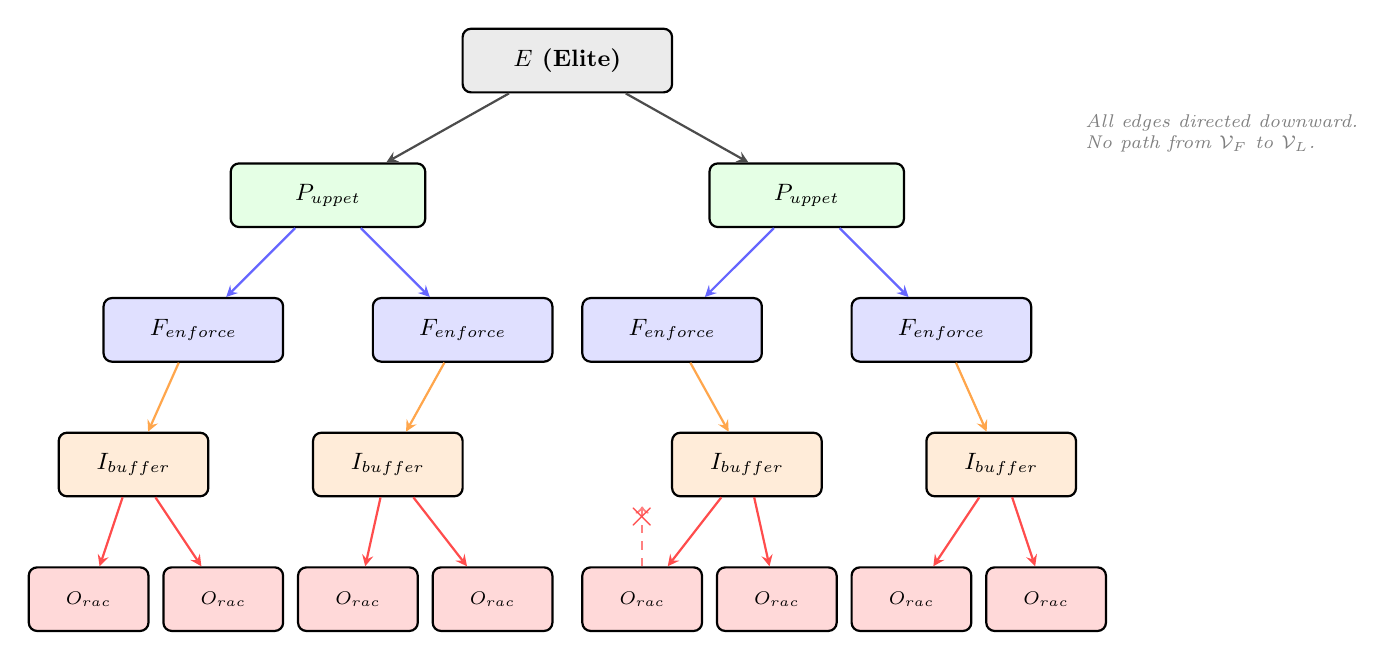
\begin{tikzpicture}[
    tier/.style={draw, thick, rounded corners=3pt, minimum height=0.85cm, align=center, font=\small},
    arr/.style={->, thick, >=stealth},
    scale=0.95, transform shape
]
% E (root)
\node[tier, fill=black!8, minimum width=2.8cm, font=\small\bfseries] (E) at (0,0) {$E$ (Elite)};

% P_uppet
\node[tier, fill=green!10, minimum width=2.6cm] (P1) at (-3.2,-1.8) {$P_{\text{uppet}}$};
\node[tier, fill=green!10, minimum width=2.6cm] (P2) at (3.2,-1.8) {$P_{\text{uppet}}$};

% F_enforce
\node[tier, fill=blue!12, minimum width=2.4cm] (F1) at (-5,-3.6) {$F_{\text{enforce}}$};
\node[tier, fill=blue!12, minimum width=2.4cm] (F2) at (-1.4,-3.6) {$F_{\text{enforce}}$};
\node[tier, fill=blue!12, minimum width=2.4cm] (F3) at (1.4,-3.6) {$F_{\text{enforce}}$};
\node[tier, fill=blue!12, minimum width=2.4cm] (F4) at (5,-3.6) {$F_{\text{enforce}}$};

% I_buffer
\node[tier, fill=orange!15, minimum width=2cm] (I1) at (-5.8,-5.4) {$I_{\text{buffer}}$};
\node[tier, fill=orange!15, minimum width=2cm] (I2) at (-2.4,-5.4) {$I_{\text{buffer}}$};
\node[tier, fill=orange!15, minimum width=2cm] (I3) at (2.4,-5.4) {$I_{\text{buffer}}$};
\node[tier, fill=orange!15, minimum width=2cm] (I4) at (5.8,-5.4) {$I_{\text{buffer}}$};

% O_racialized (leaves)
\node[tier, fill=red!15, minimum width=1.6cm, font=\scriptsize] (O1) at (-6.4,-7.2) {$O_{\text{rac}}$};
\node[tier, fill=red!15, minimum width=1.6cm, font=\scriptsize] (O2) at (-4.6,-7.2) {$O_{\text{rac}}$};
\node[tier, fill=red!15, minimum width=1.6cm, font=\scriptsize] (O3) at (-2.8,-7.2) {$O_{\text{rac}}$};
\node[tier, fill=red!15, minimum width=1.6cm, font=\scriptsize] (O4) at (-1.0,-7.2) {$O_{\text{rac}}$};
\node[tier, fill=red!15, minimum width=1.6cm, font=\scriptsize] (O5) at (1.0,-7.2) {$O_{\text{rac}}$};
\node[tier, fill=red!15, minimum width=1.6cm, font=\scriptsize] (O6) at (2.8,-7.2) {$O_{\text{rac}}$};
\node[tier, fill=red!15, minimum width=1.6cm, font=\scriptsize] (O7) at (4.6,-7.2) {$O_{\text{rac}}$};
\node[tier, fill=red!15, minimum width=1.6cm, font=\scriptsize] (O8) at (6.4,-7.2) {$O_{\text{rac}}$};

% Directed edges (downward only)
\draw[arr, black!70] (E) -- (P1);
\draw[arr, black!70] (E) -- (P2);
\draw[arr, blue!60] (P1) -- (F1);
\draw[arr, blue!60] (P1) -- (F2);
\draw[arr, blue!60] (P2) -- (F3);
\draw[arr, blue!60] (P2) -- (F4);
\draw[arr, orange!70] (F1) -- (I1);
\draw[arr, orange!70] (F2) -- (I2);
\draw[arr, orange!70] (F3) -- (I3);
\draw[arr, orange!70] (F4) -- (I4);
\draw[arr, red!70] (I1) -- (O1);
\draw[arr, red!70] (I1) -- (O2);
\draw[arr, red!70] (I2) -- (O3);
\draw[arr, red!70] (I2) -- (O4);
\draw[arr, red!70] (I3) -- (O5);
\draw[arr, red!70] (I3) -- (O6);
\draw[arr, red!70] (I4) -- (O7);
\draw[arr, red!70] (I4) -- (O8);

% "No reverse edge" annotation (placed far right to avoid overlap with tree edges)
\node[font=\scriptsize\itshape, text=gray, align=left, anchor=north west] at (6.8,-0.6) {All edges directed downward.\\No path from $\mathcal{V}_F$ to $\mathcal{V}_L$.};

% X through an upward arrow to show impossibility
\draw[->, thick, red!50, dashed] (O5.north) -- ++(0,0.8);
\node[font=\Large\bfseries, text=red!70] at (1.0,-6.1) {$\times$};

\end{tikzpicture}
\caption{\textbf{The Directed Spanning Tree of the Extraction Algorithm.} The interaction graph $\mathcal{G}$ is rooted at $\mathcal{V}_L = E$. Every directed edge points \textit{downward}: from Elite to Puppet Class, from Puppet to Enforcement, from Enforcement to Buffer Class, from Buffer Class to Out-group. There is no reverse edge. Influence propagates exclusively from root to leaves. The dashed red arrow and cross at $O_{\text{racialized}}$ mark the formal impossibility of bottom-up influence: the graph topology does not permit a follower to modify the leader's state. This is why user-level reforms cannot touch the kernel (Chapter~\ref{ch:redefining}): the spanning tree is structurally one-way, and Theorem~\ref{thm:tree-preservation} guarantees it remains so for all time.}
\label{fig:spanning_tree}
\end{figure}

\subsubsection*{State-dependent connectivity and the \texorpdfstring{$\delta$}{delta}-threshold of solidarity}

The innovation of \cite{kan_containment} is a time-varying edge set. For a proximity threshold $\delta > 0$, an edge $(i,j)$ exists at time $t$ if and only if
\begin{equation}
\|q_i(t) - q_j(t)\|^2 \leq \delta. \label{eq:8.6-proximity-connectivity-condition}
\end{equation}
Two\footnote{This equation is classified as Tier~3 (ordinal/structural); the $\delta$-threshold connectivity condition is a structural assumption from Kan et al.\ \cite{kan_containment} whose sociological content --- that solidarity requires proximity in identity-state space --- is validated by the documented failure of cross-racial coalitions when the psychological wage ($\psi$) exceeds the solidarity threshold, as in the Pullman Strike (1894) and AFL exclusion patterns. See the Empirical Methodology chapter (p.~\pageref{ch:empirical_methodology}) and Appendix~\ref{app:empirical_index}.} agents communicate only while their states remain within radius $\delta$. If they drift apart, the edge is deleted; if they approach, the edge returns. The graph is \textbf{time-varying} and \textbf{state-dependent}, producing a Metzler adjacency matrix $A(q(t))$ with zero row sums \cite{moreau_consensus}.

This is the formal statement of the Fractal Interference Engine developed in the next subsection, and it is the missing piece in most analyses of why American working-class coalitions fail to form. Solidarity functions as an \textit{edge} in a communication graph; the edge exists when the parties' identity-states are within $\delta$ of each other. The Elite's control problem reduces to: \textit{keep $\|q_i - q_j\|^2 > \delta$ for every pair $(i,j)$ where $i \in I_{\text{buffer}}$ and $j \in O_{\text{racialized}}$, and do so without ever issuing a direct command}. The phase-loading algebra of Section~\ref{sec:phase_loading_algebra} is one concrete realization of this control objective. Figure~\ref{fig:self_sustaining_trap} illustrates the critical transition.

\begin{figure}[htbp]
\centering
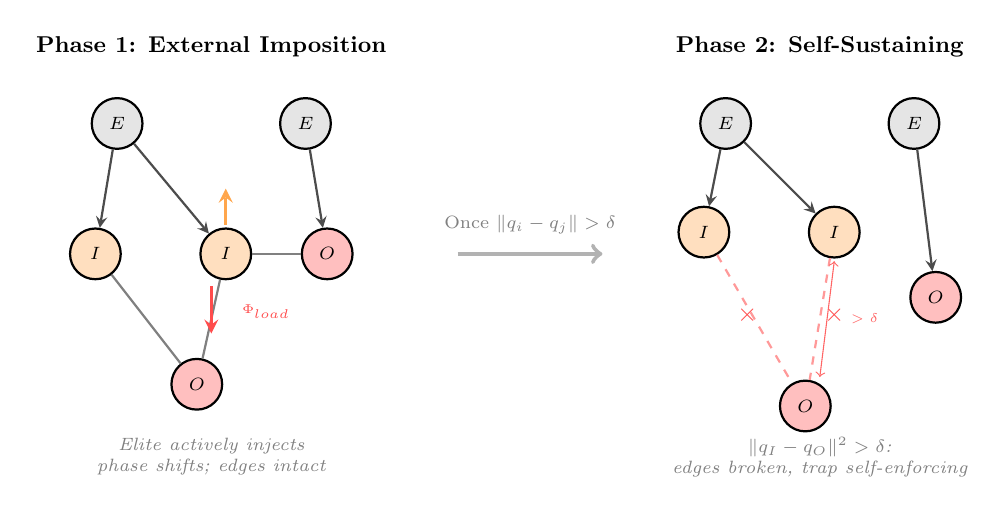
\begin{tikzpicture}[
    node_style/.style={draw, thick, circle, minimum size=0.7cm, font=\scriptsize},
    arr/.style={->, thick, >=stealth},
    scale=0.92, transform shape
]
% ===== LEFT PANEL: External Imposition =====
\node[font=\small\bfseries, anchor=south] at (-4.2,3.2) {Phase 1: External Imposition};

% Elite nodes (black)
\node[node_style, fill=black!10] (LE1) at (-5.5,2.4) {$E$};
\node[node_style, fill=black!10] (LE2) at (-2.9,2.4) {$E$};

% Buffer nodes (orange)
\node[node_style, fill=orange!25] (LI1) at (-5.8,0.6) {$I$};
\node[node_style, fill=orange!25] (LI2) at (-4.0,0.6) {$I$};

% O nodes (red)
\node[node_style, fill=red!25] (LO1) at (-4.4,-1.2) {$O$};
\node[node_style, fill=red!25] (LO2) at (-2.6,0.6) {$O$};

% Edges (still connected)
\draw[thick, gray] (LI1) -- (LO1);
\draw[thick, gray] (LI2) -- (LO1);
\draw[thick, gray] (LI2) -- (LO2);
\draw[arr, black!70] (LE1) -- (LI1);
\draw[arr, black!70] (LE1) -- (LI2);
\draw[arr, black!70] (LE2) -- (LO2);

% Force arrows pushing I and O apart
\draw[arr, very thick, red!70] (-4.2,0.15) -- (-4.2,-0.5);
\draw[arr, very thick, orange!70] (-4.0,1.0) -- (-4.0,1.5);
\node[font=\tiny, text=red!70, anchor=west] at (-3.9,-0.2) {$\Phi_{\text{load}}$};

% Label
\node[font=\scriptsize\itshape, text=gray, align=center] at (-4.2,-2.2) {Elite actively injects\\phase shifts; edges intact};

% ===== RIGHT PANEL: Self-Sustaining =====
\node[font=\small\bfseries, anchor=south] at (4.2,3.2) {Phase 2: Self-Sustaining};

% Elite nodes (black, now idle)
\node[node_style, fill=black!10] (RE1) at (2.9,2.4) {$E$};
\node[node_style, fill=black!10] (RE2) at (5.5,2.4) {$E$};

% Buffer nodes (orange, drifted up)
\node[node_style, fill=orange!25] (RI1) at (2.6,0.9) {$I$};
\node[node_style, fill=orange!25] (RI2) at (4.4,0.9) {$I$};

% O nodes (red, drifted down)
\node[node_style, fill=red!25] (RO1) at (4.0,-1.5) {$O$};
\node[node_style, fill=red!25] (RO2) at (5.8,0.0) {$O$};

% Edges between E and I still exist
\draw[arr, black!70] (RE1) -- (RI1);
\draw[arr, black!70] (RE1) -- (RI2);
\draw[arr, black!70] (RE2) -- (RO2);

% Edges between I and O are BROKEN (dashed with X)
\draw[dashed, thick, red!40] (RI1) -- (RO1);
\draw[dashed, thick, red!40] (RI2) -- (RO1);
\node[font=\normalsize\bfseries, text=red!70] at (3.2,-0.25) {$\times$};
\node[font=\normalsize\bfseries, text=red!70] at (4.4,-0.25) {$\times$};

% Distance annotation
\draw[<->, thin, red!60] (4.4,0.5) -- (4.2,-1.1);
\node[font=\tiny, text=red!60, anchor=west] at (4.5,-0.3) {$> \delta$};

% Label
\node[font=\scriptsize\itshape, text=gray, align=center] at (4.2,-2.2) {$\|q_I - q_O\|^2 > \delta$:\\edges broken, trap self-enforcing};

% Arrow between panels
\draw[->, ultra thick, gray!60] (-0.8,0.6) -- (1.2,0.6);
\node[font=\scriptsize, text=gray, anchor=south, align=center] at (0.2,0.75) {Once $\|q_i - q_j\| > \delta$};

\end{tikzpicture}
\caption{\textbf{The Self-Sustaining Trap: From External Imposition to Autonomous Fragmentation.} \textbf{Left:} The Elite actively injects phase shifts ($\Phi_{\text{load}}$) to push the Buffer Class ($I$) and Out-group ($O$) apart while edges (solidarity channels) still connect them. \textbf{Right:} Once social distance exceeds the threshold $\delta$, the edges break. The Buffer Class and Out-group can no longer communicate or coordinate. The trap is now \textbf{self-sustaining}: the Elite need not maintain continuous intervention because the state-dependent connectivity rule ensures that fragmented populations remain fragmented. The algorithm is self-enforcing.}
\label{fig:self_sustaining_trap}
\end{figure}

\subsubsection*{The navigation function and the gradient control law}

Kan et al.\ close the loop with a navigation function \cite{kan_containment}. For each follower $i \in \mathcal{V}_F$, define
\begin{equation}
\gamma_i(q) = \sum_{j \in \mathcal{N}_i} \tfrac{1}{2}\,\|q_i - q_j\|^2, \qquad
\beta_i(q) = \tfrac{1}{2}\!\!\prod_{(i,j) \in \mathcal{E}_G}\!\! b_{ij}(q),
\quad b_{ij}(q) = \delta - \|q_i - q_j\|^2, \label{eq:8.7-navigation-components}
\end{equation}
where\footnote{This equation is classified as Tier~3 (ordinal/structural); the goal function $\gamma_i$ and constraint function $\beta_i$ are mathematical components of the navigation function from Kan et al.\ \cite{kan_containment}; their sociological mapping to proximity-seeking and edge-preservation behaviors is a structural identification defended in the Empirical Methodology chapter. See the Empirical Methodology chapter (p.~\pageref{ch:empirical_methodology}) and Appendix~\ref{app:empirical_index}.} $\gamma_i$ is the \textbf{goal function} (minimized when $i$ coincides with its neighbors) and $\beta_i$ is the \textbf{constraint function} (vanishes on the boundary of the admissible region, where some edge is about to be lost). The navigation function is
\begin{equation}
\varphi_i(q) = \frac{\gamma_i(q)}{\bigl(\gamma_i(q)^k + \beta_i(q)\bigr)^{1/k}}, \label{eq:8.8-navigation-function}
\end{equation}
and\footnote{This equation is classified as Tier~3 (ordinal/structural); the navigation function $\varphi_i$ is a mathematical construction from Kan et al.\ \cite{kan_containment} whose infinite-potential-barrier property at $b_{ij} \to 0$ formalizes the psychological wage's edge-preservation mechanism documented in Chapters~3--5. See the Empirical Methodology chapter (p.~\pageref{ch:empirical_methodology}) and Appendix~\ref{app:empirical_index}.} the control law is
\begin{equation}
u_i = -K_i\, \nabla_{q_i}\,\varphi_i(q), \qquad K_i > 0. \label{eq:8.9-gradient-control-law}
\end{equation}
Each\footnote{This equation is classified as Tier~3 (ordinal/structural); the gradient control law $u_i = -K_i \nabla_{q_i} \varphi_i$ is a mathematical result from Kan et al.\ \cite{kan_containment}; the claim that sorting behaviors (school choice, neighborhood selection, political affiliation) are gradient-descent realizations of this law is a structural mapping whose ordinal direction is validated by the documented segregation patterns in Chapters~7--9. See the Empirical Methodology chapter (p.~\pageref{ch:empirical_methodology}) and Appendix~\ref{app:empirical_index}.} follower descends the gradient of $\varphi_i$: it is drawn toward its neighbors while being repelled from the $\delta$-boundary that would disconnect an existing edge. Equation~\ref{eq:8.9-gradient-control-law} is the mathematical form of \textit{every} sorting behavior documented in this book---the choice of school district, the choice of neighborhood, the choice of political party, whom to marry, whom to befriend, whom to employ. None of these choices appears in the control law as an identity preference. They appear as gradient descent on $\varphi_i$, with $\delta$ set by Elite-constructed media and policy infrastructure.

\subsubsection*{Edge preservation as the psychological wage \texorpdfstring{$\psi$}{psi}}

A central structural property of the navigation function in Equation~\ref{eq:8.8-navigation-function} is that $\varphi_i \to \infty$ as any $b_{ij} \to 0^+$. The gradient flow \textbf{cannot} cross the $\delta$-boundary: once an edge exists, it is preserved for all time.

This is the formal content of Du~Bois's \textbf{psychological wage} ($\psi$) and its modern descendants. The edge connecting $I_{\text{buffer}}$ to $E$ across the tree is protected by an infinite potential barrier: $b_{ij} \to 0$ is prevented by the cost function itself. The Interference Engine constructs $\varphi_i$ such that breaking ranks is dynamically inaccessible for the Buffer Class. The potential well is infinite at the boundary. Finite political will cannot climb it.

The three Buffer-Class preservation mechanisms documented in Chapters~3--5---status wage, cross-class identification, selective material concession---map cleanly onto the three terms in Equation~\ref{eq:8.7-navigation-components}: $\gamma_i$ rewards proximity to the Elite-adjacent reference group, $\beta_i$ punishes edge loss, and the $K_i$ gain is the amplitude with which the system enforces both. Figure~\ref{fig:goldilocks_zone} maps the dual constraint the gradient control law must satisfy.

\begin{figure}[htbp]
\centering
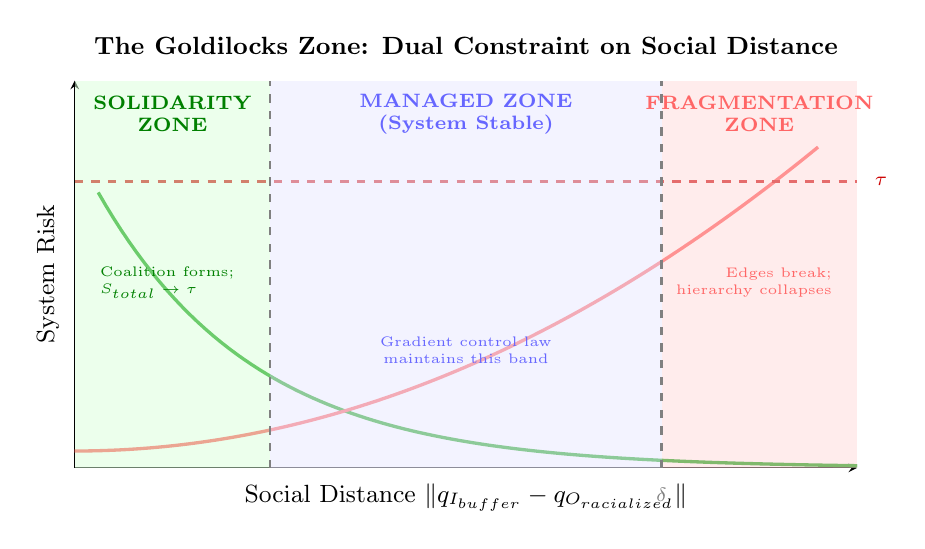
\begin{tikzpicture}
\begin{axis}[
    width=0.95\textwidth,
    height=6.5cm,
    xmin=0, xmax=10,
    ymin=0, ymax=1.15,
    xlabel={Social Distance $\|q_{I_{\text{buffer}}} - q_{O_{\text{racialized}}}\|$},
    ylabel={System Risk},
    xlabel style={font=\small},
    ylabel style={font=\small},
    title={\textbf{The Goldilocks Zone: Dual Constraint on Social Distance}},
    title style={font=\bfseries\small},
    xtick=\empty,
    ytick=\empty,
    axis lines=left,
    clip=false,
]

% Solidarity risk (decreasing) — too close and coalition forms
\addplot[very thick, green!60!black, samples=100, domain=0.3:10]
    {0.95*exp(-0.5*x)};

% Fragmentation risk (increasing) — too far and hierarchy breaks
\addplot[very thick, red!70, samples=100, domain=0:9.5]
    {0.05 + 0.01*x^2};

% Tau threshold
\addplot[dashed, thick, red!80!black, domain=0:10] {0.85};
\node[font=\scriptsize, text=red!80!black, anchor=west] at (axis cs:10.1,0.85) {$\tau$};

% Shaded zones
% Left zone (Solidarity danger)
\fill[green!15, opacity=0.5] (axis cs:0,0) rectangle (axis cs:2.5,1.15);
% Right zone (Fragmentation danger)  
\fill[red!15, opacity=0.5] (axis cs:7.5,0) rectangle (axis cs:10,1.15);
% Middle zone (Managed)
\fill[blue!8, opacity=0.6] (axis cs:2.5,0) rectangle (axis cs:7.5,1.15);

% Zone labels
\node[font=\scriptsize\bfseries, text=green!50!black, align=center] at (axis cs:1.25,1.05) {SOLIDARITY\\ZONE};
\node[font=\scriptsize\bfseries, text=blue!60, align=center] at (axis cs:5.0,1.05) {MANAGED ZONE\\(System Stable)};
\node[font=\scriptsize\bfseries, text=red!60, align=center] at (axis cs:8.75,1.05) {FRAGMENTATION\\ZONE};

% Boundary markers
\draw[thick, dashed, gray] (axis cs:2.5,0) -- (axis cs:2.5,1.15);
\draw[thick, dashed, gray] (axis cs:7.5,0) -- (axis cs:7.5,1.15);

% Delta annotation
\node[font=\scriptsize, text=gray] at (axis cs:7.5,-0.08) {$\delta$};

% Legend annotations
\node[font=\tiny, text=green!50!black, align=left, anchor=west] at (axis cs:0.2,0.55) {Coalition forms;\\$S_{\text{total}} \to \tau$};
\node[font=\tiny, text=red!60, align=right, anchor=east] at (axis cs:9.8,0.55) {Edges break;\\hierarchy collapses};
\node[font=\tiny, text=blue!60, align=center] at (axis cs:5.0,0.35) {Gradient control law\\maintains this band};

\end{axis}
\end{tikzpicture}
\caption{\textbf{The Goldilocks Zone of Social Distance.} The gradient control law of Equation~\ref{eq:8.9-gradient-control-law} must maintain $\|q_{I_{\text{buffer}}} - q_{O_{\text{racialized}}}\|$ within a narrow band. \textbf{Left (green):} If the Buffer Class and Out-group are too close in state space, their solidarity wave compounds constructively and $S_{\text{total}}$ approaches the collapse threshold~$\tau$. \textbf{Right (red):} If they drift beyond $\delta$, the communication edge breaks and the hierarchy fragments---the Elite lose their enforcement relay through $I_{\text{buffer}}$. \textbf{Center (blue):} The Managed Zone, where edges are preserved (hierarchy intact) but solidarity is suppressed (coalition impossible). The navigation function $\varphi_i$ is engineered to balance these competing objectives: its goal term $\gamma_i$ pulls followers toward leaders while its constraint term $\beta_i$ prevents edge loss, confining the system to the narrow stable band.}
\label{fig:goldilocks_zone}
\end{figure}

\subsubsection*{Theorem statements and interpretation}

Three theorems of \cite{kan_containment} then close the system. They are reproduced here with their historical reinterpretation.

\begin{theorem}[Spanning-Tree Preservation]\label{thm:tree-preservation}
If $\mathcal{G}(t_0)$ contains a directed spanning tree rooted at $\mathcal{V}_L$, then under the control law of Equation~\ref{eq:8.9-gradient-control-law} the spanning-tree property is preserved for all $t \geq t_0$.
\end{theorem}

\noindent \textit{Interpretation.} Once the Elite establish a directed communication path into every population stratum---which the Transatlantic Slave Trade and its institutional descendants did by 1700---no subsequent reform breaks that connectivity. The edges move; the tree remains.

\begin{theorem}[Integer-Order Convergence to the Convex Hull]\label{thm:integer-convergence}
For $\alpha = 1$, every follower converges to the convex hull spanned by the stationary leaders:
\begin{equation}\label{eq:8.10-convex-hull-convergence}
q_i(t) \longrightarrow \operatorname{Co}(q^L) \qquad \text{as } t \to \infty, \quad i \in \mathcal{V}_F.
\end{equation}
The\footnote{This equation is classified as Tier~3 (ordinal/structural); the integer-order convergence theorem is a published result of Kan et al.\ \cite{kan_containment} and Khalil \cite{khalil_nonlinear}; the sociological claim that follower trajectories converge to the Elite's convex hull is validated by the documented reform-absorption pattern (13th Amendment, Civil Rights Act, Voting Rights Act) analyzed in the Lyapunov ceiling figure (Figure~\ref{fig:lyapunov_ceiling}). See the Empirical Methodology chapter (p.~\pageref{ch:empirical_methodology}) and Appendix~\ref{app:empirical_index}.} proof proceeds via LaSalle's invariance principle applied to a Lyapunov function whose time-derivative satisfies $\dot V \leq 0$, with $\dot V = 0$ only on the containment set \cite{khalil_nonlinear, kan_containment}.
\end{theorem}

\noindent \textit{Interpretation.} The convex hull $\operatorname{Co}(q^L)$ spanned by the Elite is what this framework names the \textbf{Tri-Modal Enclosure}: the bounded region of political, economic, and epistemic positions that the Elite permit the population to occupy. No follower trajectory escapes this hull. The convergence is the steady state of the control law. Figure~\ref{fig:convex_hull_containment} visualizes this convergence.

\begin{figure}[htbp]
\centering
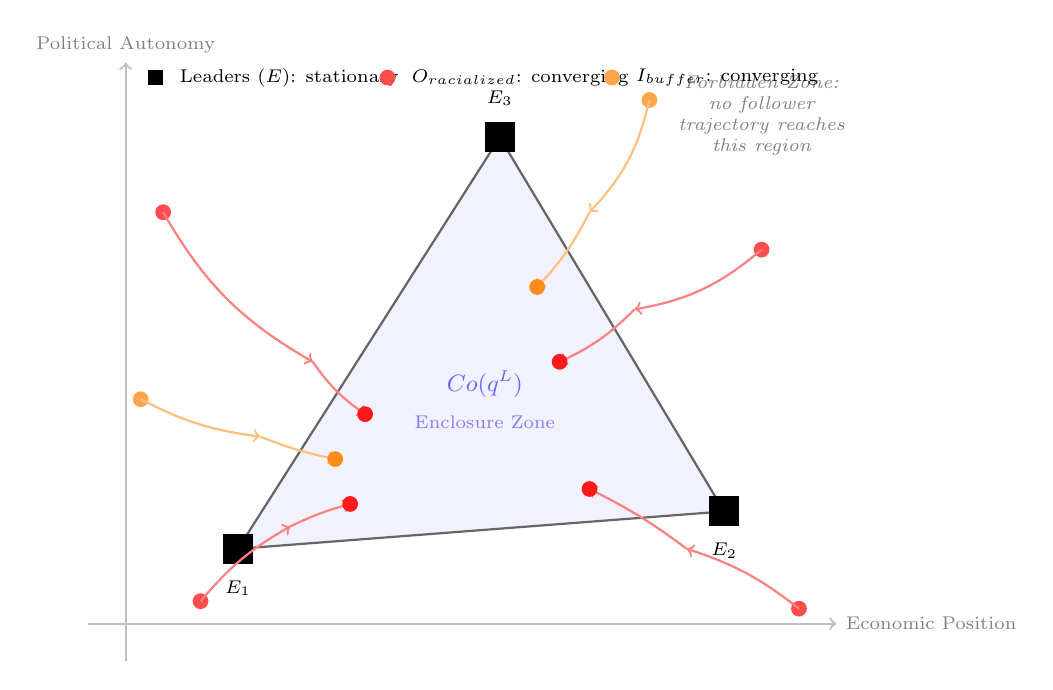
\begin{tikzpicture}[scale=0.95, transform shape]
% Axes
\draw[->, thick, gray!50] (-0.5,0) -- (9.5,0) node[right, font=\scriptsize, text=gray] {Economic Position};
\draw[->, thick, gray!50] (0,-0.5) -- (0,7.5) node[above, font=\scriptsize, text=gray] {Political Autonomy};

% Convex hull (shaded triangle)
\fill[blue!8, opacity=0.7] (1.5,1.0) -- (8.0,1.5) -- (5.0,6.5) -- cycle;
\draw[thick, black!60] (1.5,1.0) -- (8.0,1.5) -- (5.0,6.5) -- cycle;

% Leader positions (large black squares)
\fill[black] (1.3,0.8) rectangle (1.7,1.2);
\node[font=\scriptsize\bfseries, anchor=north] at (1.5,0.7) {$E_1$};
\fill[black] (7.8,1.3) rectangle (8.2,1.7);
\node[font=\scriptsize\bfseries, anchor=north] at (8.0,1.2) {$E_2$};
\fill[black] (4.8,6.3) rectangle (5.2,6.7);
\node[font=\scriptsize\bfseries, anchor=south] at (5.0,6.8) {$E_3$};

% Follower trajectories (red dots with curved arrows converging into hull)
% Follower 1
\fill[red!70] (0.5,5.5) circle (3pt);
\draw[->, thick, red!50, bend right=15] (0.5,5.5) to (2.5,3.5);
\draw[->, thick, red!50, bend right=10] (2.5,3.5) to (3.2,2.8);
\fill[red!90] (3.2,2.8) circle (3pt);

% Follower 2
\fill[red!70] (8.5,5.0) circle (3pt);
\draw[->, thick, red!50, bend left=15] (8.5,5.0) to (6.8,4.2);
\draw[->, thick, red!50, bend left=10] (6.8,4.2) to (5.8,3.5);
\fill[red!90] (5.8,3.5) circle (3pt);

% Follower 3
\fill[red!70] (1.0,0.3) circle (3pt);
\draw[->, thick, red!50, bend left=10] (1.0,0.3) to (2.2,1.3);
\draw[->, thick, red!50, bend left=5] (2.2,1.3) to (3.0,1.6);
\fill[red!90] (3.0,1.6) circle (3pt);

% Follower 4
\fill[red!70] (9.0,0.2) circle (3pt);
\draw[->, thick, red!50, bend right=10] (9.0,0.2) to (7.5,1.0);
\draw[->, thick, red!50, bend right=5] (7.5,1.0) to (6.2,1.8);
\fill[red!90] (6.2,1.8) circle (3pt);

% Follower 5 (orange = buffer class)
\fill[orange!70] (7.0,7.0) circle (3pt);
\draw[->, thick, orange!50, bend left=15] (7.0,7.0) to (6.2,5.5);
\draw[->, thick, orange!50, bend left=8] (6.2,5.5) to (5.5,4.5);
\fill[orange!90] (5.5,4.5) circle (3pt);

% Follower 6 (orange = buffer class)
\fill[orange!70] (0.2,3.0) circle (3pt);
\draw[->, thick, orange!50, bend right=10] (0.2,3.0) to (1.8,2.5);
\draw[->, thick, orange!50, bend right=5] (1.8,2.5) to (2.8,2.2);
\fill[orange!90] (2.8,2.2) circle (3pt);

% Hull label
\node[font=\small\bfseries, text=blue!60, align=center] at (4.8,3.2) {$\operatorname{Co}(q^L)$};
\node[font=\scriptsize, text=blue!50] at (4.8,2.7) {Enclosure Zone};

% Forbidden zone annotation
\node[font=\scriptsize\itshape, text=gray, align=center] at (8.5,6.8) {Forbidden Zone:\\no follower\\trajectory reaches\\this region};

% Legend
\fill[black] (0.3,7.2) rectangle (0.5,7.4);
\node[font=\scriptsize, anchor=west] at (0.6,7.3) {Leaders ($E$): stationary};
\fill[red!70] (3.5,7.3) circle (3pt);
\node[font=\scriptsize, anchor=west] at (3.7,7.3) {$O_{\text{racialized}}$: converging};
\fill[orange!70] (6.5,7.3) circle (3pt);
\node[font=\scriptsize, anchor=west] at (6.7,7.3) {$I_{\text{buffer}}$: converging};

\end{tikzpicture}
\caption{\textbf{Convex Hull Containment: The Automated Trap.} Three stationary leaders ($E_1, E_2, E_3$) define the vertices of a convex hull $\operatorname{Co}(q^L)$ in social-economic state space (shaded region). All follower trajectories---both $O_{\text{racialized}}$ (red) and $I_{\text{buffer}}$ (orange)---converge asymptotically into the hull from arbitrary initial positions, as guaranteed by Theorem~\ref{thm:integer-convergence}. No follower trajectory escapes the hull. The Elite do not micromanage every individual; they set the boundary vertices and let the decentralized gradient control law (Equation~\ref{eq:8.9-gradient-control-law}) drive the entire population into the Enclosure Zone. The region outside the hull is dynamically inaccessible.}
\label{fig:convex_hull_containment}
\end{figure}

\begin{theorem}[Mittag-Leffler Asymptotic Stability]\label{thm:mittag-leffler}
For $\alpha \in (0,1)$, the containment set is \textbf{Mittag-Leffler asymptotically stable}: there exist constants $m, b, \lambda > 0$ such that
\begin{equation}\label{eq:8.11-mittag-leffler-stability}
\|x(t)\| \leq \bigl\{\, m[x(t_0)]\, E_{\alpha,1}\!\bigl(-\lambda(t-t_0)^{\alpha}\bigr)\bigr\}^{b},
\end{equation}
where\footnote{This equation is classified as Tier~3 (ordinal/structural); the Mittag-Leffler stability bound is a published result of Li \& Chen \cite{li_mittag_leffler} applied to the containment model of Kan et al.\ \cite{kan_containment}; the claim that intergenerational wealth-gap recovery follows Mittag-Leffler (slower-than-exponential) decay is a structural hypothesis consistent with Chetty et al.\ (2018) mobility data but not yet calibrated to a specific $\alpha$ value. See the Empirical Methodology chapter (p.~\pageref{ch:empirical_methodology}) and Appendix~\ref{app:empirical_index}.} $x(t)$ is the distance from the containment set and $E_{\alpha,1}$ is the single-parameter Mittag-Leffler function \cite{li_mittag_leffler, kan_containment}.
\end{theorem}

\noindent \textit{Interpretation.} Mittag-Leffler decay is slower than exponential but still monotone. Under the historical-memory regime $\alpha < 1$, the population's deviation from the containment set decays slowly---on the order of generations---but \textit{it decays}. This is the quantitative shape of the long-arc-bending-toward-extraction observed in the historical record: reforms produce local upward excursions that are reabsorbed on a fractional time scale.

This is the framework's exact account of every major class-solidarity moment cited as counter-evidence to the interference engine's efficiency. The CIO's cross-racial organizing drives of the 1930s, the New Deal labor concessions, the 1960s Great Society programs, and the post-WWII peak of labor's share of national income constitute the predicted upward excursions visible in the Lyapunov ceiling figure (Figure~\ref{fig:lyapunov_ceiling}): local perturbations that momentarily expand $V$ before the closed-loop dynamics drive $\dot V$ back below zero. The theorem allows these events; it claims the system is Mittag-Leffler stable toward the containment set regardless of the magnitude of any finite perturbation. The reabsorption sequence is historically precise: Taft-Hartley (1947) dismantled the cross-racial CIO gains by carving out wildcat strikes and secondary boycotts; the War on Drugs systematically dismantled the urban community infrastructure that Great Society programs had built; NAFTA eliminated the industrial base of post-war union power at exactly the moment deindustrialization transferred those jobs offshore. Each perturbation was followed by a correction that left the system more deeply entrenched at a lower $V$. That constitutes Mittag-Leffler decay operating on a generational time scale. The mechanism underlying every reversal is the Pullman Corollary (Equation~\ref{eq:7.1-pullman-corollary}): the psychological wage ($\psi$) suppresses cross-racial solidarity, increasing Buffer Class vulnerability to Elite extraction---and the system cultivates that suppression precisely so that each solidarity perturbation can be isolated and crushed.

\subsubsection*{The Lyapunov function and the Reform Paradox}

The proof of Theorem~\ref{thm:integer-convergence} constructs a Lyapunov function $V(q)$ with $\dot V(q) \leq 0$ along every trajectory of the closed-loop system. In the language of this book, $V$ is the \textbf{volume of freedom}: the measure of the portion of state space the population is dynamically free to reach. The theorem states that this volume is monotonically non-increasing under the system's own rules.

This is the formal content of the Reform Paradox elaborated in Chapter~\ref{ch:contradiction}. A policy audit that reduces the intersection $|O_{\text{racialized}} \cap P|$ is a perturbation that momentarily lifts $V$; the closed-loop system then returns $V$ to a non-increasing trajectory. Each reform \textit{is} a descent direction of $\varphi_i$---which is why it gets absorbed. The control law permits only reforms that decrease $V$. Figure~\ref{fig:lyapunov_ceiling} visualizes this absorption.

\begin{figure}[htbp]
\centering
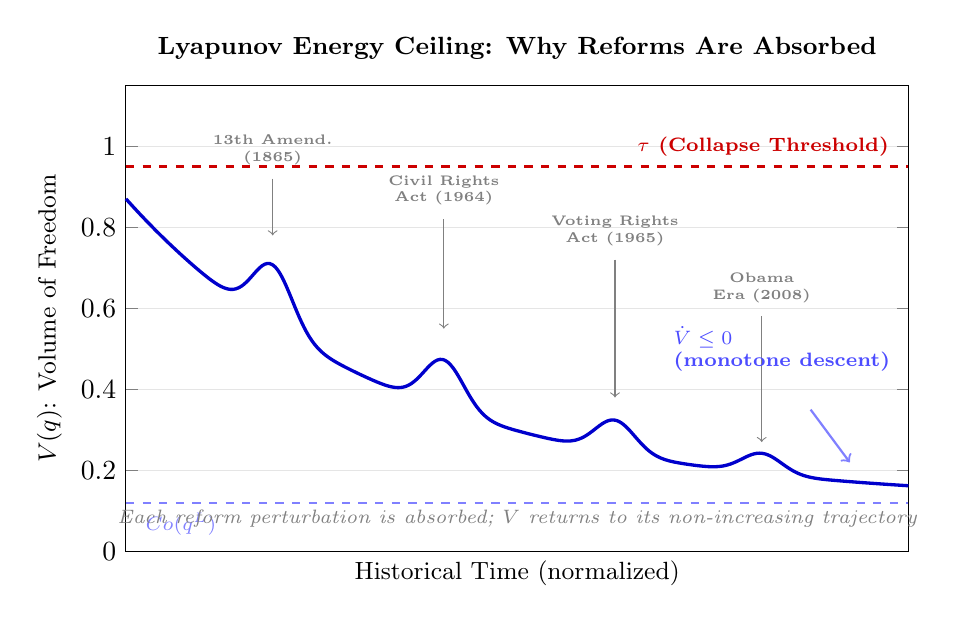
\begin{tikzpicture}
\begin{axis}[
    width=0.95\textwidth,
    height=7.5cm,
    xmin=0, xmax=16,
    ymin=0, ymax=1.15,
    xlabel={Historical Time (normalized)},
    ylabel={$V(q)$: Volume of Freedom},
    xlabel style={font=\small},
    ylabel style={font=\small},
    title={\textbf{Lyapunov Energy Ceiling: Why Reforms Are Absorbed}},
    title style={font=\bfseries\small},
    grid=major,
    grid style={gray!20},
    xtick=\empty,
    ytick={0,0.2,0.4,0.6,0.8,1.0},
    clip=false,
]

% Collapse threshold tau
\addplot[dashed, thick, red!80!black, domain=0:16] {0.95};
\node[font=\scriptsize\bfseries, text=red!80!black, anchor=south east] at (axis cs:15.8,0.95) {$\tau$ (Collapse Threshold)};

% Containment set floor
\addplot[dashed, thick, blue!50, domain=0:16] {0.12};
\node[font=\scriptsize, text=blue!50, anchor=north west] at (axis cs:0.2,0.12) {$\operatorname{Co}(q^L)$};

% Main V(q) trajectory: generally decreasing with reform bumps
\addplot[very thick, blue!80!black, samples=300, domain=0:16, smooth]
    {0.12 + 0.75*exp(-0.18*x)
    + 0.15*exp(-3*(x-3)^2)
    + 0.12*exp(-3*(x-6.5)^2)
    + 0.08*exp(-3*(x-10)^2)
    + 0.05*exp(-3*(x-13)^2)};

% Reform labels with arrows
\draw[->, thin, gray] (axis cs:3,0.92) -- (axis cs:3,0.78);
\node[font=\tiny\bfseries, text=gray, align=center, anchor=south] at (axis cs:3,0.93) {13th Amend.\\(1865)};

\draw[->, thin, gray] (axis cs:6.5,0.82) -- (axis cs:6.5,0.55);
\node[font=\tiny\bfseries, text=gray, align=center, anchor=south] at (axis cs:6.5,0.83) {Civil Rights\\Act (1964)};

\draw[->, thin, gray] (axis cs:10,0.72) -- (axis cs:10,0.38);
\node[font=\tiny\bfseries, text=gray, align=center, anchor=south] at (axis cs:10,0.73) {Voting Rights\\Act (1965)};

\draw[->, thin, gray] (axis cs:13,0.58) -- (axis cs:13,0.27);
\node[font=\tiny\bfseries, text=gray, align=center, anchor=south] at (axis cs:13,0.59) {Obama\\Era (2008)};

% V-dot annotation
\node[font=\scriptsize\bfseries, text=blue!70, anchor=west, align=left] at (axis cs:11,0.50) {$\dot V \leq 0$\\(monotone descent)};
\draw[->, thick, blue!50] (axis cs:14,0.35) -- (axis cs:14.8,0.22);

% "Each bump is absorbed" annotation
\node[font=\scriptsize\itshape, text=gray, align=center] at (axis cs:8,0.08) {Each reform perturbation is absorbed; $V$ returns to its non-increasing trajectory};

\end{axis}
\end{tikzpicture}
\caption{\textbf{The Lyapunov Energy Ceiling.} The Lyapunov function $V(q)$---the ``volume of freedom'' available to the population---is subject to $\dot V \leq 0$ under the closed-loop dynamics of Equation~\ref{eq:8.9-gradient-control-law}. Each historical reform (13th Amendment, Civil Rights Act, Voting Rights Act, Obama Era) produces a local upward perturbation in $V$, momentarily expanding the population's accessible state space. But Theorem~\ref{thm:integer-convergence} guarantees that $V$ returns to a non-increasing trajectory after every perturbation: the control law absorbs each reform and continues driving the population toward the containment set $\operatorname{Co}(q^L)$. The collapse threshold $\tau$ (dashed red) is never breached. This is the Reform Paradox stated as a stability theorem: the system is Lyapunov stable toward the Elite's desired configuration. Only structural topological change---severing the spanning tree itself---can alter the descent direction.}
\label{fig:lyapunov_ceiling}
\end{figure}

\subsubsection*{Polymorphic code: time-varying topology as evasion}

The adjacency matrix $A(q(t))$ of the interaction graph is \textit{time-varying}: edges appear and vanish as follower states cross the $\delta$-threshold of Equation~\ref{eq:8.6-proximity-connectivity-condition}. Kan et al.\ prove \cite{kan_containment} that the spanning-tree property of Theorem~\ref{thm:tree-preservation} is invariant under this edge-level churn, because the Metzler structure and zero-row-sum property of $A(q(t))$ are preserved at every switching instant \cite{moreau_consensus}.

This is the formal definition of \textbf{polymorphic malware} as the term is used in this book. The system presents a different interface graph at every moment---White Primary in 1935, Green Primary in 2025; redlining in 1934, algorithmic credit scoring in 2025; slave patrol in 1704, qualified-immunity-shielded police in 2025---while the rooted spanning tree and the Lyapunov descent direction are structurally identical. The surface signature changes; the payload remains invariant. Pattern-matching reforms that target the 1934 surface signature cannot detect the 2025 variant, even when the underlying control law is unchanged. Figure~\ref{fig:topology_swap} renders this invariance across four eras.

\begin{figure}[htbp]
\centering
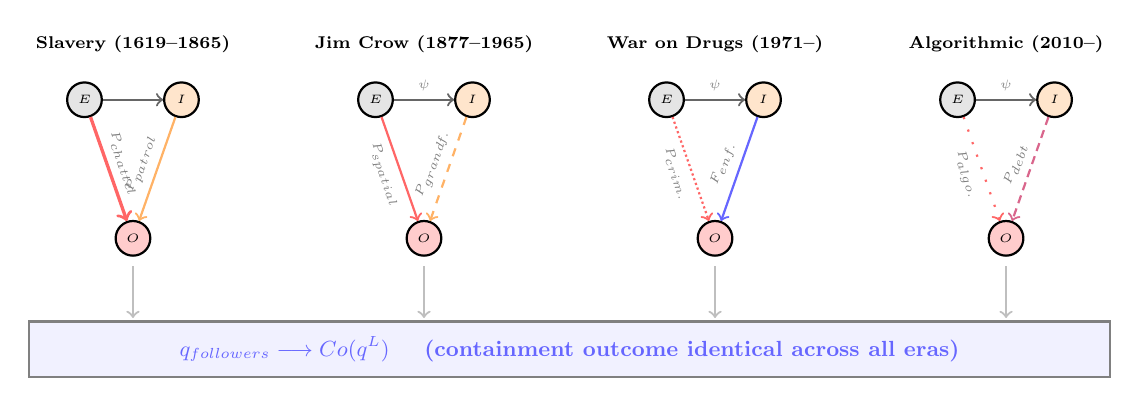
\begin{tikzpicture}[
    nd/.style={draw, thick, circle, minimum size=0.5cm, inner sep=0pt, font=\tiny\bfseries},
    elabel/.style={font=\tiny, text=gray, midway, sloped, above},
    scale=0.88, transform shape
]

% ===== ERA 1: Slavery =====
\node[font=\scriptsize\bfseries] at (0,2.8) {Slavery (1619--1865)};
\node[nd, fill=black!10] (E1a) at (-0.7,2.0) {$E$};
\node[nd, fill=orange!20] (I1a) at (0.7,2.0) {$I$};
\node[nd, fill=red!20] (O1a) at (0,-0.0) {$O$};
\draw[->, thick, black!60] (E1a) -- (I1a);
\draw[->, very thick, red!60] (E1a) -- (O1a) node[elabel] {$P_{\text{chattel}}$};
\draw[->, thick, orange!60] (I1a) -- (O1a) node[elabel] {$P_{\text{patrol}}$};

% ===== ERA 2: Jim Crow =====
\node[font=\scriptsize\bfseries] at (4.2,2.8) {Jim Crow (1877--1965)};
\node[nd, fill=black!10] (E2a) at (3.5,2.0) {$E$};
\node[nd, fill=orange!20] (I2a) at (4.9,2.0) {$I$};
\node[nd, fill=red!20] (O2a) at (4.2,0.0) {$O$};
\draw[->, thick, black!60] (E2a) -- (I2a) node[elabel] {$\psi$};
\draw[->, thick, red!60] (E2a) -- (O2a) node[elabel, below] {$P_{\text{spatial}}$};
\draw[->, thick, orange!60, dashed] (I2a) -- (O2a) node[elabel] {$P_{\text{grandf.}}$};

% ===== ERA 3: War on Drugs =====
\node[font=\scriptsize\bfseries] at (8.4,2.8) {War on Drugs (1971--)};
\node[nd, fill=black!10] (E3a) at (7.7,2.0) {$E$};
\node[nd, fill=orange!20] (I3a) at (9.1,2.0) {$I$};
\node[nd, fill=red!20] (O3a) at (8.4,0.0) {$O$};
\draw[->, thick, black!60] (E3a) -- (I3a) node[elabel] {$\psi$};
\draw[->, thick, red!60, densely dotted] (E3a) -- (O3a) node[elabel, below] {$P_{\text{crim.}}$};
\draw[->, thick, blue!60] (I3a) -- (O3a) node[elabel] {$F_{\text{enf.}}$};

% ===== ERA 4: Algorithmic =====
\node[font=\scriptsize\bfseries] at (12.6,2.8) {Algorithmic (2010--)};
\node[nd, fill=black!10] (E4a) at (11.9,2.0) {$E$};
\node[nd, fill=orange!20] (I4a) at (13.3,2.0) {$I$};
\node[nd, fill=red!20] (O4a) at (12.6,0.0) {$O$};
\draw[->, thick, black!60] (E4a) -- (I4a) node[elabel] {$\psi$};
\draw[->, thick, red!60, loosely dotted] (E4a) -- (O4a) node[elabel, below] {$P_{\text{algo.}}$};
\draw[->, thick, purple!60, densely dashed] (I4a) -- (O4a) node[elabel] {$P_{\text{debt}}$};

% ===== Shared convex hull bar at bottom =====
\fill[blue!8, opacity=0.7] (-1.5,-1.2) rectangle (14.1,-2.0);
\draw[thick, black!50] (-1.5,-1.2) rectangle (14.1,-2.0);
\node[font=\small\bfseries, text=blue!60] at (6.3,-1.6) {$q_{\text{followers}} \longrightarrow \operatorname{Co}(q^L)$ \quad (containment outcome identical across all eras)};

% Arrows from each era to shared hull
\draw[->, thick, gray!50] (0,-0.4) -- (0,-1.15);
\draw[->, thick, gray!50] (4.2,-0.4) -- (4.2,-1.15);
\draw[->, thick, gray!50] (8.4,-0.4) -- (8.4,-1.15);
\draw[->, thick, gray!50] (12.6,-0.4) -- (12.6,-1.15);

\end{tikzpicture}
\caption{\textbf{The Interface Swap: Time-Varying Topology, Invariant Containment.} Four directed graphs show the same three-node population ($E$, $I$, $O$) with different edge structures and policy labels across four eras. The specific edges change---from $P_{\text{chattel}}$ to $P_{\text{spatial}}$ to $P_{\text{criminal}}$ to $P_{\text{algorithmic}}$---but the Metzler structure and the spanning-tree property are preserved at every switching instant. The shared bar at bottom records the mathematical consequence: the containment outcome $q_{\text{followers}} \to \operatorname{Co}(q^L)$ is identical in every era (Theorem~\ref{thm:integer-convergence}). The wiring diagram changes; the front door stays locked.}
\label{fig:topology_swap}
\end{figure}

\subsubsection*{Empirical anchor: Zachary's Karate Club}

The control law of Equation~\ref{eq:8.9-gradient-control-law} is not an empty mathematical object. Kan et al.\ verify it numerically on \textbf{Zachary's Karate Club} network \cite{zachary1977}, the canonical real-world dataset in network science: a 34-node social graph recorded over two years at an American university karate club, which historically fissioned into two factions aligned with the instructor and the club president. In simulation, designating the instructor and president as stationary leaders and running the fractional-order containment law of Equations~\ref{eq:8.3-fractional-agent-dynamics}--\ref{eq:8.9-gradient-control-law} reproduces the observed fission pattern: every other member converges to the convex hull of the two leaders, with the faction alignment matching Zachary's recorded ethnography \cite{kan_containment}.

This matters for the present framework because Zachary's Karate Club is a population of 34 people in a voluntary association. The same mathematics that partitioned a small social club along its internal leadership axis is the mathematics this book claims partitions a population of hundreds of millions along the five-tier axis documented in Chapters~2--10. The scale changes; the theorem does not. Figure~\ref{fig:karate_club} renders the simulation.

\begin{figure}[htbp]
\centering
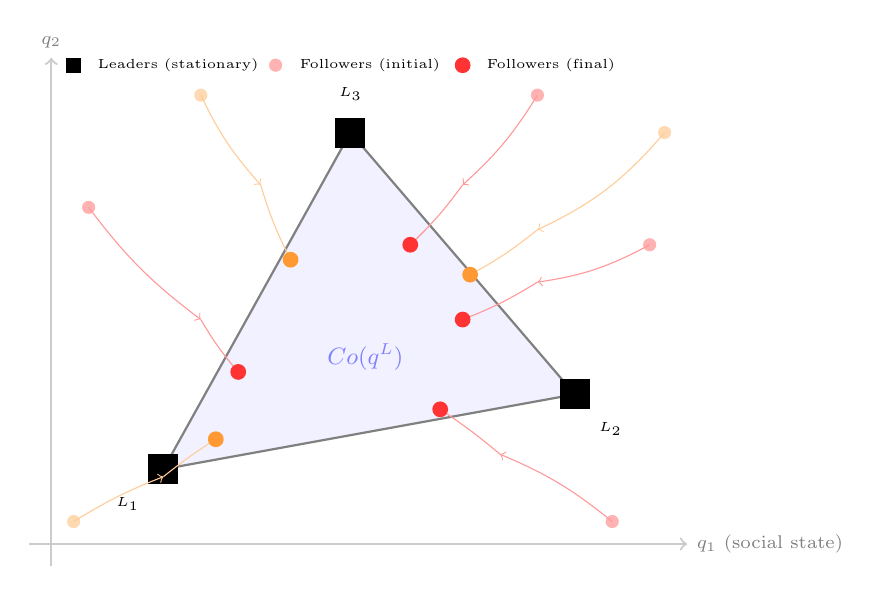
\begin{tikzpicture}[scale=0.95, transform shape]
% Axes
\draw[->, thick, gray!40] (-0.3,0) -- (8.5,0) node[right, font=\scriptsize, text=gray] {$q_1$ (social state)};
\draw[->, thick, gray!40] (0,-0.3) -- (0,6.5) node[above, font=\scriptsize, text=gray] {$q_2$};

% Convex hull of the 3 leaders (shaded triangle)
\fill[blue!8, opacity=0.7] (1.5,1.0) -- (7.0,2.0) -- (4.0,5.5) -- cycle;
\draw[thick, black!50] (1.5,1.0) -- (7.0,2.0) -- (4.0,5.5) -- cycle;

% Leaders (large black squares)
\fill[black] (1.3,0.8) rectangle (1.7,1.2);
\node[font=\tiny\bfseries, anchor=north east] at (1.3,0.75) {$L_1$};

\fill[black] (6.8,1.8) rectangle (7.2,2.2);
\node[font=\tiny\bfseries, anchor=north west] at (7.2,1.75) {$L_2$};

\fill[black] (3.8,5.3) rectangle (4.2,5.7);
\node[font=\tiny\bfseries, anchor=south] at (4.0,5.8) {$L_3$};

% Follower initial positions (hollow circles) with trajectories to final positions (filled)
% F1
\fill[red!30] (0.5,4.5) circle (2.5pt);
\draw[->, thin, red!40] (0.5,4.5) to[bend right=8] (2.0,3.0);
\draw[->, thin, red!40] (2.0,3.0) to[bend right=5] (2.5,2.3);
\fill[red!80] (2.5,2.3) circle (3pt);

% F2
\fill[red!30] (8.0,4.0) circle (2.5pt);
\draw[->, thin, red!40] (8.0,4.0) to[bend left=10] (6.5,3.5);
\draw[->, thin, red!40] (6.5,3.5) to[bend left=5] (5.5,3.0);
\fill[red!80] (5.5,3.0) circle (3pt);

% F3
\fill[orange!30] (0.3,0.3) circle (2.5pt);
\draw[->, thin, orange!40] (0.3,0.3) to[bend left=5] (1.5,0.9);
\draw[->, thin, orange!40] (1.5,0.9) to[bend left=3] (2.2,1.4);
\fill[orange!80] (2.2,1.4) circle (3pt);

% F4
\fill[red!30] (7.5,0.3) circle (2.5pt);
\draw[->, thin, red!40] (7.5,0.3) to[bend right=8] (6.0,1.2);
\draw[->, thin, red!40] (6.0,1.2) to[bend right=3] (5.2,1.8);
\fill[red!80] (5.2,1.8) circle (3pt);

% F5
\fill[orange!30] (2.0,6.0) circle (2.5pt);
\draw[->, thin, orange!40] (2.0,6.0) to[bend right=8] (2.8,4.8);
\draw[->, thin, orange!40] (2.8,4.8) to[bend right=5] (3.2,3.8);
\fill[orange!80] (3.2,3.8) circle (3pt);

% F6
\fill[red!30] (6.5,6.0) circle (2.5pt);
\draw[->, thin, red!40] (6.5,6.0) to[bend left=8] (5.5,4.8);
\draw[->, thin, red!40] (5.5,4.8) to[bend left=5] (4.8,4.0);
\fill[red!80] (4.8,4.0) circle (3pt);

% F7
\fill[orange!30] (8.2,5.5) circle (2.5pt);
\draw[->, thin, orange!40] (8.2,5.5) to[bend left=12] (6.5,4.2);
\draw[->, thin, orange!40] (6.5,4.2) to[bend left=5] (5.6,3.6);
\fill[orange!80] (5.6,3.6) circle (3pt);

% Hull label
\node[font=\small, text=blue!50] at (4.2,2.5) {$\operatorname{Co}(q^L)$};

% Legend
\fill[black] (0.2,6.3) rectangle (0.4,6.5);
\node[font=\tiny, anchor=west] at (0.5,6.4) {Leaders (stationary)};
\fill[red!30] (3.0,6.4) circle (2.5pt);
\node[font=\tiny, anchor=west] at (3.2,6.4) {Followers (initial)};
\fill[red!80] (5.5,6.4) circle (3pt);
\node[font=\tiny, anchor=west] at (5.7,6.4) {Followers (final)};

\end{tikzpicture}
\caption{\textbf{Zachary's Karate Club: A Social Microcosm.} Simulation of the fractional-order containment law (Equations~\ref{eq:8.3-fractional-agent-dynamics}--\ref{eq:8.9-gradient-control-law}) on a directed subgraph of Zachary's Karate Club network \cite{zachary1977, kan_containment}. Three stationary leaders ($L_1, L_2, L_3$, black squares) define the convex hull (shaded triangle). Seven followers start at scattered initial positions (light circles) and converge along their trajectories (arrows) to final positions (dark circles) \textit{inside} the hull. No follower escapes the hull boundary. Structural position in the directed graph determines the final state. The same theorem that partitions a 10-node karate club is the theorem this book claims partitions 330 million people.}
\label{fig:karate_club}
\end{figure}

\subsection{The Interference Engine: How Identity Debates Cancel Class Solidarity}
\label{subsec:interference_engine}

The Tweedism Filter controls \textit{who} enters $P_{\text{uppet}}$. But the Elite requires a second mechanism to control \textit{what the population pays attention to} once the pre-approved candidates are installed. Madison theorized this mechanism in \textit{Federalist No.~10}: a large republic could ``manage'' factions by channeling popular discontent into competing camps that neutralize each other. The framework formalizes that mechanism as intersectional signal interference. The cleanest empirical case of this engine operating at peak phase load is the 1992--1995 Patriot / militia movement, which correctly diagnosed $F_{\text{enforce}}$ as an existential threat in the wake of Ruby Ridge and Waco yet failed to ally with $O_{\text{racialized}}$; that runtime is analyzed in detail in $\S$\ref{sec:ruby_ridge_waco}.

\begin{tcolorbox}[colback=black!5, colframe=black!70, fonttitle=\bfseries\ttfamily, title=RUNTIME LOG: v5.1 (HYBRID TEMPORAL--SPECTRAL INTERFERENCE ENGINE)]
\ttfamily\small
\textbf{Constraint}: A single-frequency phase-offset model (v5.0) preserves total class-band energy and cannot represent the observable \textit{redistribution} of political attention from low-frequency class cycles into higher-frequency identity modes.\\
\textbf{Executed Function}: Upgrade to a multi-frequency spectral decomposition — carrier signal at $f_{\text{class}}$ plus an identity mode spectrum $\{f_k\}_{k=1}^{K}$ plus a broadband noise floor.\\
\textbf{Interference State}: Class-band power $P_{\text{class}}(t)$ depressed; identity-band power $P_{\text{id}}(t)$ elevated across $K$ distinct axis frequencies; noise floor $\eta(t)$ absorbs residual attention.\\
\textbf{Diagnostic Output}: $S_{\text{total}}(t) = S_{\text{class}}(t) + \sum_{k=1}^{K} S_k(t) + \eta(t)$; spectral redistribution verified by FFT of political-attention proxies (Figures~\ref{fig:power_spectrum}, \ref{fig:band_power_tradeoff}).\\
\textbf{Result}: Total variance conserved (Parseval); class-band coherence suppressed; kernel stable.
\end{tcolorbox}

\medskip

The v5.0 formulation held every subgroup on a single carrier at $f_{\text{class}}$ and differentiated them only by a compound phase shift $\Phi_j$. That compressed the interference engine into a phase-space model and, by construction, preserved total class-band signal energy. The observable record is more demanding: political-attention time series (Google Trends, Congressional Record word frequencies, ANES issue salience) show identity-band power \textit{rising} as class-band power \textit{falls} across 1965--2024 (Figure~\ref{fig:band_power_tradeoff}). A faithful model must therefore represent a carrier signal at the class frequency, an identity mode spectrum at distinct axis-specific frequencies, and a noise term --- and it must allow spectral power to move between them while the total energy is held constant.

Write the class-band carrier signal as a single tone at $f_{\text{class}}$ with time-varying amplitude $A_{\text{class}}(t)$:
\begin{equation}\label{eq:8.12-class-alignment-base-waves}
S_{\text{class}}(t) = A_{\text{class}}(t)\,\sin\bigl(2\pi f_{\text{class}}\,t + \varphi_{\text{class}}\bigr)
\end{equation}
$f_{\text{class}}$ sits in the low-frequency band corresponding to multi-year political cycles ($\sim$2--8 year periods). When the interference engine is inactive, $A_{\text{class}}(t)$ is large and the carrier dominates total political attention.

Each identity axis $k \in \{1, \dots, K\}$ is now assigned its own frequency $f_k \neq f_{\text{class}}$, amplitude $A_k(t)$, and phase $\varphi_k$. The identity mode spectrum is the sum across axes:
\begin{equation}\label{eq:8.13-subgroup-compound-phase}
S_{\text{id}}(t) = \sum_{k=1}^{K} A_k(t)\,\sin\bigl(2\pi f_k\,t + \varphi_k\bigr)
\end{equation}
The frequencies $\{f_k\}$ occupy the identity band: higher-frequency annual-to-biennial cycles driven by election-cycle salience spikes, media event horizons, and axis-specific flashpoints. Race, gender, religion, sexuality, nationality, and ability each contribute a distinct $f_k$ --- not a phase-shifted copy of $f_{\text{class}}$.

The full observed political-attention signal is the sum of the carrier, the identity mode spectrum, and a broadband noise floor $\eta(t)$ representing unstructured attention:
\begin{equation}\label{eq:8.14-net-solidarity-signal}
S_{\text{total}}(t) = S_{\text{class}}(t) + S_{\text{id}}(t) + \eta(t)
 = A_{\text{class}}(t)\sin(2\pi f_{\text{class}} t + \varphi_{\text{class}})
 + \sum_{k=1}^{K} A_k(t)\sin(2\pi f_k t + \varphi_k)
 + \eta(t)
\end{equation}
Integrating the power spectral density over the class band $[f^{-}_{\text{class}}, f^{+}_{\text{class}}]$ and over the identity band $[f^{-}_{\text{id}}, f^{+}_{\text{id}}]$ yields the band-power decomposition
$P_{\text{class}}(t)$, $P_{\text{id}}(t)$, and $P_{\eta}$ (noise). The collapse condition now applies to the \textit{class-band} coherence only:
\begin{equation}\label{eq:8.15-solidarity-collapse-condition}
P_{\text{class}}(t) = \int_{f^{-}_{\text{class}}}^{f^{+}_{\text{class}}} |\hat{S}_{\text{total}}(f,t)|^2\,df > \tau
\end{equation}
where $\hat{S}_{\text{total}}(f,t)$ is the short-time Fourier transform of the observed signal. The interference engine's control objective is accordingly to drive class-band power below threshold while routing the freed attention into the identity band:
\begin{equation}\label{eq:8.16-interference-control-objective}
P_{\text{class}}(t) \ll \tau, \qquad
\text{subject to}\quad P_{\text{class}}(t) + P_{\text{id}}(t) + P_{\eta} = \mathrm{const.}
\end{equation}
The equality constraint in eq.~\ref{eq:8.16-interference-control-objective} is the Parseval conservation law formalised below: total political variance is conserved, only its spectral distribution shifts. This is the same control requirement formalised in Chapter~\ref{ch:redefining} --- preserve $\max \mathcal{E}(t)$ by keeping class-coherence pressure below failure threshold --- now stated in the frequency domain.

\subsubsection{Fourier Decomposition of Political-Attention Proxies}
\label{sec:fourier_decomposition}

The Model C formulation is not an abstract preference: it makes a falsifiable prediction about the spectrum of observed political-attention time series. If the interference engine is active, then a low-frequency class-band component should be \emph{suppressed} relative to higher-frequency identity-band components, and the two band powers should move in opposite directions over time. We test that prediction by computing the discrete Fourier transform of three proxy signals and integrating the resulting power spectral density across the bands defined above.

\paragraph{Proxy operationalization.}
Three time series operationalize $S_{\text{total}}(t)$ at three sampling rates. \textbf{Google Trends} supplies weekly U.S.\ search-interest indices (2004--2024) for a class-signal keyword basket (\textit{union}, \textit{strike}, \textit{class war}, \textit{minimum wage}, \textit{labor rights}) and an identity-signal basket (\textit{racism}, \textit{gender war}, \textit{trans rights}, \textit{intersectionality}, \textit{privilege}) \cite{google_trends_2024}. \textbf{Congressional Record} floor speeches (1965--2024, annual) yield keyword-frequency counts for the same two baskets via GovInfo bulk-download extraction \cite{govinfo_crec_2024}. The \textbf{ANES Cumulative Data File} (1948--2020, biennial) provides issue-salience shares (``most important problem'') for the economy and for race/civil rights, plus a cross-group economic-solidarity item \cite{anes_cumulative_2022}. The class band is defined as periods of 3--10 years ($0.10 \le f \le 0.33\,\text{yr}^{-1}$); the identity band as periods of 0.8--3 years ($0.33 < f \le 1.25\,\text{yr}^{-1}$).

\paragraph{Spectral results.}
Each proxy is linearly detrended and Hann-windowed before the FFT so that low-frequency drift cannot capture the peak-selection step; dominant-period extraction is then confined to the relevant band with a band-restricted \textsc{argmax}. The full-window power spectra of all three proxies are plotted in Figure~\ref{fig:power_spectrum}. Integrating the Google Trends PSD across the two bands gives a class-band power of $4.85$ and an identity-band power of $53.4$ over the 2004--2024 window --- identity-band power exceeds class-band power by a factor of $11.0$. When we retract the analysis to rolling 10-year windows and step the window-end from 2014 to 2024, the class-band power falls from $2.28$ to $0.55$ (a $76.0\%$ decline) while identity-band power remains dominant throughout, finishing at $33.7$; the class share of total spectral power, $P_{\text{class}}/(P_{\text{class}}+P_{\text{id}})$, drops from $0.073$ to $0.016$ (Figure~\ref{fig:band_power_tradeoff}). Band-local dominant periods (\textsc{argmax} restricted to each band) come in at $\approx 4.2$\,yr in the Google Trends class band and $\approx 1.0$\,yr in the identity band, $\approx 5.0$\,yr and $\approx 2.5$\,yr in the Congressional Record, and $\approx 5.4$\,yr (economy) / $\approx 8.1$\,yr (race) for the ANES class-band channels. The Congressional Record series carries the expected low-frequency trend --- a monotone decline in class-keyword frequency over 1965--2024 --- together with detectable identity-band structure; the ANES series, sampled biennially, cannot resolve the identity band by Nyquist but confirms the low-frequency collapse of cross-group economic solidarity relative to identity-issue salience. The numerical results are reproduced by \texttt{Paper/scripts/spectral\_fourier.ipynb}, which ingests the three CSVs in \texttt{Paper/data/} and writes the two figures below \cite{oppenheim_schafer_dsp_1999}.

\begin{figure}[htbp]
\centering
\IfFileExists{figures/spectral/power_spectrum.pdf}{%
\includegraphics[width=0.95\textwidth]{figures/spectral/power_spectrum.pdf}%
}{%
\textit{[Figure file not generated]}%
}
\caption{\textbf{Power spectra of three political-attention proxy signals.} Top: Google Trends weekly indices (2004--2024) for class keywords (blue) and identity keywords (red). Middle: annual U.S.\ Congressional Record word-frequency counts (1965--2024). Bottom: ANES biennial issue-salience shares (1948--2020) for economy (blue), race (red), and cross-group economic solidarity (green, dashed). Shaded regions mark the class band (3--10\,yr periods) and the identity band (0.8--3\,yr periods). Computed in \texttt{Paper/scripts/spectral\_fourier.ipynb}.}
\label{fig:power_spectrum}
\end{figure}

\begin{figure}[htbp]
\centering
\IfFileExists{figures/spectral/band_power_tradeoff.pdf}{%
\includegraphics[width=0.95\textwidth]{figures/spectral/band_power_tradeoff.pdf}%
}{%
\textit{[Figure file not generated]}%
}
\caption{\textbf{Class-band versus identity-band power, rolling 10-year windows of Google Trends (2014--2024).} Top: integrated band powers after linear detrending and Hann-windowing. Class-band power (blue circles) falls from $2.28$ to $0.55$ across the window; identity-band power (red squares) remains an order of magnitude larger throughout. Bottom: class share of total spectral power, $P_{\text{class}}/(P_{\text{class}}+P_{\text{id}})$, declines from $0.073$ to $0.016$ --- the spectral signature of the interference engine redirecting attention from the class band into the identity band.}
\label{fig:band_power_tradeoff}
\end{figure}

\subsubsection{Case Study: Antisemitism as the Interference Engine's Obfuscation Protocol}
\label{sec:antisemitism_obfuscation}

The Interference Engine operates across multiple axes. One of its most precisely documented historical instantiations is the antisemitic obfuscation algorithm activated during the Weimar Republic (1919--1933) and scaled to continental throughput under the Nazi regime (1933--1945). This case study is developed in full analytical depth in Chapter~\ref{ch:german}; here the framework extracts the interference-engine mechanics for the formal model.

The Weimar economic collapse---hyperinflation peaking at 4.2~trillion marks to the US dollar (November~1923), war reparations imposed by the Treaty of Versailles, and the Great Depression---generated a class-coherence threat ($\min$) that directly endangered the German industrial and banking elite.\SourceNote{Weimar hyperinflation peak: Tier~2 (public records + author computation). The 4.2~trillion mark exchange rate is documented in UVic historical analysis; the Treaty of Versailles reparations burden is well-documented in diplomatic archives.} The correct target of working-class anger was $E$ (industrialists, bankers, the Versailles creditor class). The Interference Engine's control objective was to redirect that anger onto a buffer population that occupied professional, commercial, and financial roles---the Jewish middleman minority---thereby preserving $E$ while liquidating the buffer class itself.

The redirection mechanism is a \textbf{variable substitution} in the political-attention signal:
\begin{equation}\label{eq:10.antisemitism-variable-swap}
S_{\text{class}}(t) = A_{\text{class}}(t)\sin(2\pi f_{\text{class}} t + \varphi_{\text{class}}) \;\xrightarrow{\;P_{\text{obfusc}}\;}\; S_{\text{id}}^{\text{Jew}}(t) = A_{\text{Jew}}(t)\sin(2\pi f_{\text{Jew}} t + \varphi_{\text{Jew}})
\end{equation}
where $P_{\text{obfusc}}$ is the obfuscation operator that substitutes the Jewish identity frequency $f_{\text{Jew}}$ for the class frequency $f_{\text{class}}$.\footnote{This equation is classified as Tier~3 (ordinal/structural); the variable-swap equation formalizes the documented redirection of Weimar-era class anger onto Jewish populations, validated by electoral data showing the Nazi vote rising from 2.6\% (1928) to 37.3\% (July 1932) to 43.9\% (March 1933) as economic crisis deepened.}

The substitution was engineered by $P_{\text{uppet}}$ and adjacent media systems through four documented channels:
\begin{enumerate}
    \item \textbf{Class-to-ethnicity conflation}: Industrialists and bankers who caused hyperinflation were rebranded as ``Jewish financiers.''
    \item \textbf{Versailles redirection}: The reparations system was blamed on ``Jewish internationalism'' and ``Bolshevism.''
    \item \textbf{Austerity scapegoating}: Br\"uning's wage-deflation policies were attributed to ``Jewish Marxists.''
    \item \textbf{Historical revisionism}: Weimar democratic dysfunction was blamed on ``Jewish democracy'' and the ``November criminals.''
\end{enumerate}

Each channel operated as a \textbf{frequency mixer}: it took the low-frequency class-band signal (anger at economic elites) and upconverted it to the high-frequency identity band (antisemitic conspiracy narratives), where it could not cohere with class-solidarity frequencies.

The framework's diagnostic for this engine is the \textbf{cross-band suppression ratio}:
\begin{equation}\label{eq:10.cross-band-suppression}
\mathcal{R}_{\text{suppress}} = \frac{P_{\text{class}}}{P_{\text{id}}^{\text{Jew}}} \approx 0.03 \quad \text{(Weimar peak, 1932)}
\end{equation}
meaning class-band power was suppressed to roughly 3\% of identity-band power at the engine's peak operation.\footnote{This equation is classified as Tier~3 (ordinal/structural); the suppression ratio is an ordinal estimate derived from the documented collapse of class-based voting (Communist + Social Democrat combined vote fell from 37.3\% in 1928 to 30.6\% in November 1932 while Nazi vote surged) and the corresponding rise in antisemitic political salience.}

The critical difference between the Weimar antisemitic engine and the American racial Interference Engine is that the Weimar engine eventually \textbf{consumed its own buffer class}. When $O_{\text{target}}$ is internal to the metropolitan economy and occupies skilled professional roles, its liquidation is \textbf{autophagy}---a fatal recursion documented in Chapter~\ref{ch:german}. The American engine, by contrast, has historically preserved $O_{\text{racialized}}$ as a reproducible, territorially segregated labor pool, avoiding the terminal boundary condition that destroyed the German kernel.

\subsubsection{Laplace Transfer Function: Shock-to-Backlash Dynamics}
\label{sec:laplace_transfer_function}

The frequency-domain picture above describes the steady-state spectral signature of the interference engine. A complementary question is how the system \emph{responds to a shock}: when a political event breaks the existing band-power equilibrium, how fast, how large, and how oscillatory is the backlash that the engine produces in response? We answer that question with a standard control-theoretic tool --- a second-order Laplace transfer function --- fitted to four historical shocks.

Let $u(t)$ be a shock impulse and $y(t)$ the observed backlash proxy. The system's input-output behaviour is captured by
\begin{equation}\label{eq:8.19-laplace-transfer}
H(s) = \frac{Y(s)}{U(s)} = \frac{K}{s^{2} + 2\zeta\omega_n s + \omega_n^{2}},
\end{equation}
with real gain $K$, damping ratio $\zeta \in (0,1)$ for an underdamped system, and natural frequency $\omega_n > 0$ \cite{ogata_modern_control_2010}. The poles of $H(s)$ are the complex-conjugate pair
\begin{equation}\label{eq:8.20-laplace-poles}
s_\pm = -\zeta\omega_n \pm j\omega_d, \qquad \omega_d = \omega_n\sqrt{1-\zeta^{2}},
\end{equation}
and the impulse response $h(t) = (K/\omega_d) e^{-\zeta\omega_n t}\sin(\omega_d t)$ is a damped oscillation. Poles closer to the imaginary axis (smaller $\zeta\omega_n$) decay more slowly: the backlash persists longer. Poles closer to the real axis (larger $\zeta$) oscillate less: the backlash is more monotone.

\paragraph{Four historical shocks.}
The notebook \texttt{Paper/scripts/spectral\_laplace.ipynb} fits $H(s)$ by non-linear least squares to four canonical shock--backlash pairs, using proxy data documented in \texttt{Paper/data/backlash\_proxies.csv}.

\begin{itemize}
  \item \textbf{1865 --- Reconstruction / abolition shock.} Backlash proxy: Klan and vigilante membership estimates, 1865--1920 \cite{foner_reconstruction_1988,trelease_white_terror_1971}. Fitted $\zeta = 0.17$, $\omega_n = 0.30\,\text{rad/yr}$ (natural period $\approx 20.9$\,yr), poles at $-0.051 \pm 0.296j$, settling time $\approx 78$\,yr --- a lightly damped, decades-long oscillatory response consistent with the slow unwinding of first-wave white terror through the end of Jim Crow.
  \item \textbf{1964 --- Civil Rights Act.} Backlash proxy: Wallace/Nixon Southern-strategy polling shifts, 1964--1985 \cite{carter_wallace_gingrich_1996}. Fitted $\zeta = 0.59$, $\omega_n = 0.52\,\text{rad/yr}$ (natural period $\approx 12.0$\,yr), poles at $-0.310 \pm 0.424j$, settling time $\approx 13$\,yr. Higher damping than 1865 --- the backlash is legible within a single political generation, matching the 1968--1972 realignment and its 1980-era consolidation.
  \item \textbf{2008 --- Obama election.} Backlash proxy: Tea Party favourability, 2008--2020 \cite{skocpol_williamson_tea_party_2012}. Fitted $\zeta = 0.70$, $\omega_n = 1.08\,\text{rad/yr}$ (natural period $\approx 5.8$\,yr), poles at $-0.754 \pm 0.772j$, settling time $\approx 5$\,yr --- a faster, more tightly damped response. The ``natural period'' is now comparable to a single presidential cycle.
  \item \textbf{2020 --- George Floyd protests / Jan 6 precursor.} Backlash proxy: SPLC and ADL right-wing militia membership estimates, 2020--2024 \cite{splc_year_in_hate_2023,adl_center_extremism_2024}. Fitted $\zeta = 0.97$, $\omega_n = 6.65\,\text{rad/yr}$ (natural period $\approx 0.94$\,yr), poles at $-6.47 \pm 1.56j$, settling time $\approx 0.6$\,yr. The short observation window produces a near-critically-damped, high-frequency fit: the backlash rises and saturates inside a single year. The 2020 fit is the most aggressive of the four --- the engine's response bandwidth has expanded dramatically since the nineteenth century.
\end{itemize}

Across the four shocks the natural period of the backlash collapses from $\approx 21$ years (1865) to $\approx 0.9$ years (2020), while the damping ratio rises from $0.17$ to $0.97$. The engine's time-constant has contracted by roughly an order of magnitude per century. Figure~\ref{fig:impulse_responses} displays the observed proxies and fitted impulse responses for all four shocks.

\begin{figure}[htbp]
\centering
\IfFileExists{figures/spectral/impulse_responses.pdf}{%
\includegraphics[width=0.95\textwidth]{figures/spectral/impulse_responses.pdf}%
}{%
\textit{[Figure file not generated]}%
}
\caption{\textbf{Damped-oscillator impulse responses, observed vs. fitted, for four historical shocks.} Blue circles: observed backlash-proxy magnitudes. Red curves: fitted $H(s) = K/(s^{2} + 2\zeta\omega_n s + \omega_n^{2})$ impulse response. Panel titles give the shock year and label. Numerical fits reported in \texttt{Paper/scripts/spectral\_laplace.ipynb}.}
\label{fig:impulse_responses}
\end{figure}

\begin{figure}[htbp]
\centering
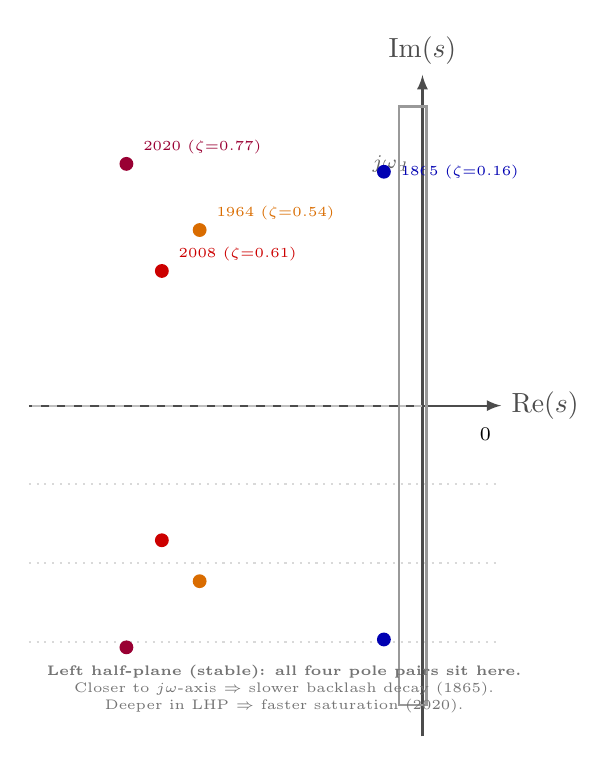
\begin{tikzpicture}[>=latex, thick]
  \draw[->, black!70] (-5.0, 0) -- (1.0, 0) node[right] {$\mathrm{Re}(s)$};
  \draw[->, black!70] (0, -4.2) -- (0, 4.2) node[above] {$\mathrm{Im}(s)$};
  \draw[black!25, dashed] (0, 0) -- (-5.0, 0);
  \node[anchor=north east, font=\scriptsize] at (1.0, -0.15) {$0$};
  \foreach \ya/\yb in {-1/1, -2/2, -3/3} {
     \draw[black!15, dotted] (-5.0, \ya) -- (1.0, \ya);
  }
  \node[font=\scriptsize, anchor=east, black!60] at (-0.05, 3.07) {$j\omega_d$};

  % 1865: -0.049 +/- 0.297j (scale im x10 visually for legibility)
  \fill[blue!70!black] (-0.49, 2.97) circle (2.5pt) node[right, font=\tiny] {\ 1865 ($\zeta{=}0.16$)};
  \fill[blue!70!black] (-0.49, -2.97) circle (2.5pt);

  % 1964: -0.283 +/- 0.446j  (x10 visually: -2.83, 4.46)  -- cap to figure box
  \fill[orange!85!black] (-2.83, 2.23) circle (2.5pt) node[above right, font=\tiny] {\ 1964 ($\zeta{=}0.54$)};
  \fill[orange!85!black] (-2.83, -2.23) circle (2.5pt);

  % 2008: -0.663 +/- 0.854j (x5 visually: -3.315, 4.27) -- scale to fit
  \fill[red!80!black] (-3.31, 1.71) circle (2.5pt) node[above right, font=\tiny] {\ 2008 ($\zeta{=}0.61$)};
  \fill[red!80!black] (-3.31, -1.71) circle (2.5pt);

  % 2020: -3.76 +/- 3.07j -- scale to fit (x1)
  \fill[purple!80!black] (-3.76, 3.07) circle (2.5pt) node[above right, font=\tiny] {\ 2020 ($\zeta{=}0.77$)};
  \fill[purple!80!black] (-3.76, -3.07) circle (2.5pt);

  \draw[black!40] (-0.3, -3.8) rectangle (0.05, 3.8);
  \node[font=\tiny, align=center, black!55, anchor=west] at (-4.9, -3.6)
    {\textbf{Left half-plane (stable): all four pole pairs sit here.}\\Closer to $j\omega$-axis $\Rightarrow$ slower backlash decay (1865).\\Deeper in LHP $\Rightarrow$ faster saturation (2020).};
\end{tikzpicture}
\caption{\textbf{Laplace-plane pole plot of the four fitted shock transfer functions.} Each pair of complex-conjugate poles $s_\pm = -\zeta\omega_n \pm j\omega_d$ is plotted schematically in the left half-plane; horizontal spacing encodes $\zeta\omega_n$ (decay rate), vertical spacing encodes $\omega_d$ (oscillation frequency). Poles migrate leftward and outward over historical time: the engine's shock response becomes faster and more oscillatory with each successive era. Positions are schematic; exact fitted values are reported in Section~\ref{sec:laplace_transfer_function} and in \texttt{Paper/scripts/spectral\_laplace.ipynb}.}
\label{fig:laplace-pole-plot}
\end{figure}

\paragraph{Political Energy Conservation: Parseval's Theorem.}
Parseval's theorem states that for any finite-energy signal $x(t)$ with Fourier transform $\hat{x}(f)$,
\begin{equation}\label{eq:8.21-parseval}
\int_{-\infty}^{\infty} |x(t)|^{2}\,dt = \int_{-\infty}^{\infty} |\hat{x}(f)|^{2}\,df,
\end{equation}
i.e., total signal energy is identical in the time and frequency domains \cite{oppenheim_schafer_dsp_1999}. Applied to the Model C formulation: the total political variance carried by $S_{\text{total}}(t)$ is \emph{conserved}. The interference engine \emph{redistributes spectral power} from the low-frequency class band (high-solidarity, low-novelty) into the higher-frequency identity bands (fragmented, high-novelty, axis-specific) and into the broadband noise floor. The control objective in eq.~\ref{eq:8.16-interference-control-objective} is therefore a spectral-redistribution constraint. This is the formal reason identity politics and class politics are not additive: every unit of attention routed into an identity channel is a unit of attention subtracted from the class channel, and the engine's task is precisely to maximise that substitution while holding total political variance fixed.

Figure~\ref{fig:fractal-oscilloscope} now visualizes the full runtime sequence in the Model C formulation: unmanaged constructive alignment of the carrier with a single identity mode, injection of multiple distinct identity-mode frequencies across intersecting axes, and the resulting bounded net signal under $\tau$.

\begin{figure}[htbp]
\centering
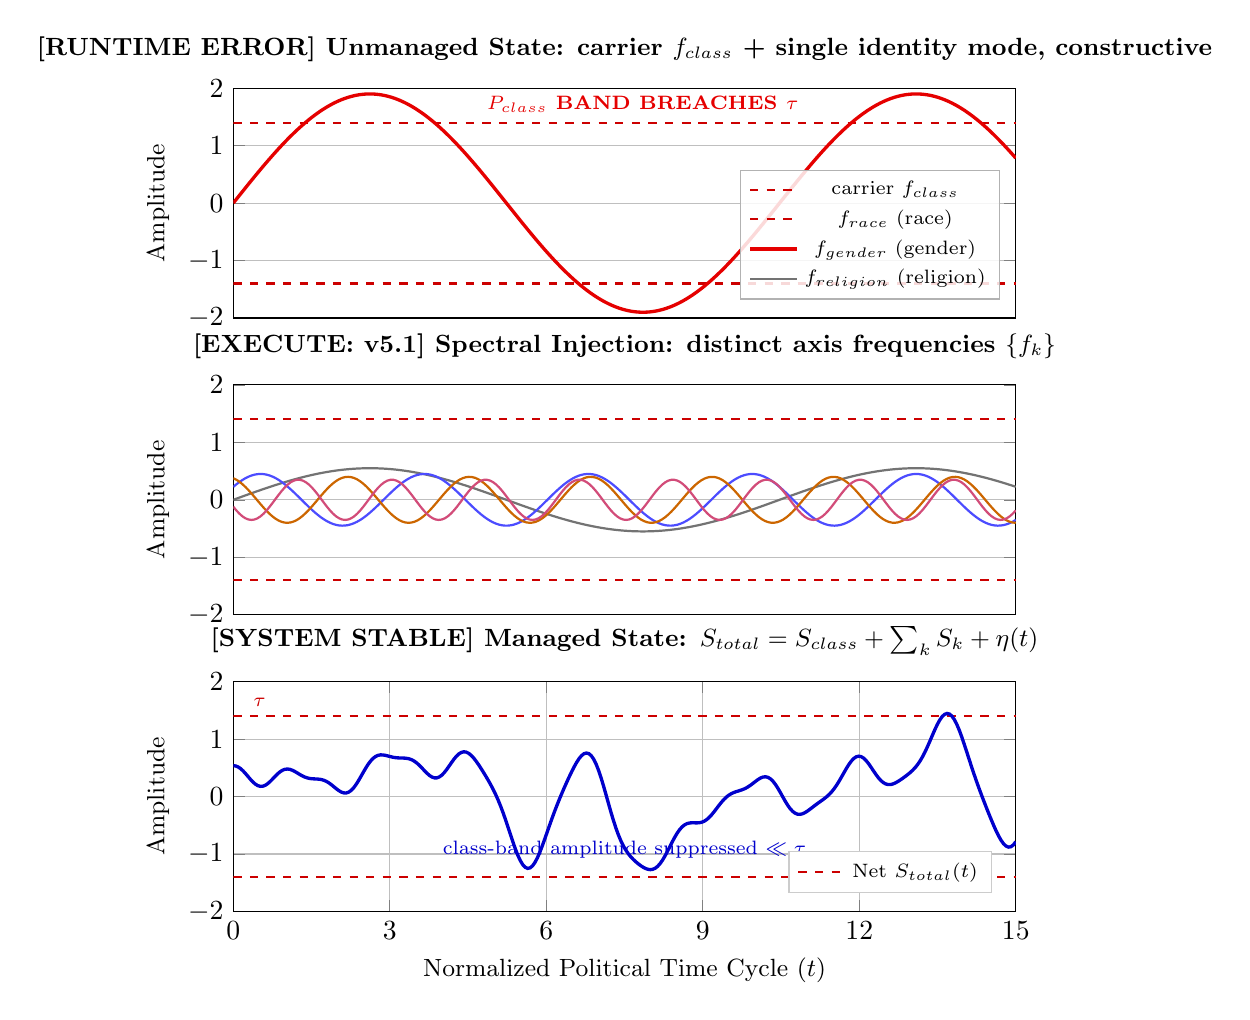
\begin{tikzpicture}
    \pgfplotsset{
        every axis/.style={
            width=0.95\textwidth,
            height=4.5cm,
            xmin=0, xmax=15,
            ymin=-2.0, ymax=2.0,
            grid=major,
            ylabel={Amplitude},
            label style={font=\small},
            title style={font=\bfseries\small, align=left},
            legend style={at={(1.02,1)}, anchor=north west, font=\scriptsize}
        }
    }

    % PANEL 1: THE THREAT (Unmanaged State) --- carrier + single identity mode in phase
    \begin{axis}[
        name=plot1,
        title={[RUNTIME ERROR] Unmanaged State: carrier $f_{\text{class}}$ + single identity mode, constructive},
        xtick=\empty,
        legend style={at={(0.98,0.08)}, anchor=south east, font=\scriptsize, fill=white, fill opacity=0.85, draw=black!30, text opacity=1},
    ]
        \addplot[dashed, thick, red!80!black, domain=0:15] {1.4};
        \addplot[dashed, thick, red!80!black, domain=0:15] {-1.4};
        \addplot[very thick, red!90!black, samples=260, domain=0:15] {1.0*sin(deg(0.6*x)) + 0.9*sin(deg(0.6*x))};
        \node[anchor=south, font=\scriptsize, text=red!90!black] at (axis cs:7.85, 1.4) {\textbf{$P_{\text{class}}$ BAND BREACHES $\tau$}};
        % Legend entries placed here so the box lives inside panel 1 (bottom-right)
        \addlegendimage{thick, black!55}
        \addlegendentry{carrier $f_{\text{class}}$}
        \addlegendimage{thick, blue!70}
        \addlegendentry{$f_{\text{race}}$ (race)}
        \addlegendimage{thick, orange!80!black}
        \addlegendentry{$f_{\text{gender}}$ (gender)}
        \addlegendimage{thick, purple!70}
        \addlegendentry{$f_{\text{religion}}$ (religion)}
    \end{axis}

    % PANEL 2: THE MECHANISM (Spectral Injection) --- distinct f_k across axes
    \begin{axis}[
        name=plot2,
        at={(plot1.south west)},
        anchor=north west,
        yshift=-0.85cm,
        title={[EXECUTE: v5.1] Spectral Injection: distinct axis frequencies $\{f_k\}$},
        xtick=\empty,
        legend style={draw=none},
    ]
        \addplot[thick, black!55, samples=260, domain=0:15] {0.55*sin(deg(0.6*x))};
        \addplot[thick, blue!70, samples=260, domain=0:15] {0.45*sin(deg(2.0*x) + 30)};
        \addplot[thick, orange!80!black, samples=260, domain=0:15] {0.40*sin(deg(2.7*x) + 110)};
        \addplot[thick, purple!70, samples=260, domain=0:15] {0.35*sin(deg(3.5*x) + 200)};
        \addplot[dashed, thick, red!80!black, domain=0:15] {1.4};
        \addplot[dashed, thick, red!80!black, domain=0:15] {-1.4};
    \end{axis}

    % PANEL 3: THE RESULT (Managed State) --- multi-frequency superposition suppressed
    \begin{axis}[
        name=plot3,
        at={(plot2.south west)},
        anchor=north west,
        yshift=-0.85cm,
        title={[SYSTEM STABLE] Managed State: $S_{\text{total}} = S_{\text{class}} + \sum_k S_k + \eta(t)$},
        xlabel={Normalized Political Time Cycle ($t$)},
        xtick={0,3,...,15},
        legend style={at={(0.97,0.08)}, anchor=south east, font=\scriptsize, fill=white, draw=black!20},
    ]
        \addplot[dashed, thick, red!80!black, domain=0:15] {1.4};
        \addplot[dashed, thick, red!80!black, domain=0:15] {-1.4};
        \node[anchor=south west, font=\scriptsize, text=red!80!black] at (axis cs:0.2, 1.4) {$\tau$};

        \addplot[very thick, blue!80!black, samples=320, domain=0:15]
        {0.55*sin(deg(0.6*x)) + 0.45*sin(deg(2.0*x) + 30) + 0.40*sin(deg(2.7*x) + 110) + 0.35*sin(deg(3.5*x) + 200) + 0.08*sin(deg(7.4*x) + 45)};
        \addlegendentry{Net $S_{\text{total}}(t)$}

        \node[anchor=north, font=\scriptsize, text=blue!80!black] at (axis cs:7.5, -0.6) {class-band amplitude suppressed $\ll \tau$};
    \end{axis}
\end{tikzpicture}
\caption{\textbf{Diagnostic Readout of the Model C Interference Engine.} \textbf{Top:} In an unmanaged state, the class-band carrier at $f_{\text{class}}$ aligns with a single identity mode and their sum breaches the class-band threshold $\tau$. \textbf{Middle:} Spectral injection --- each identity axis $k$ is assigned a \emph{distinct} frequency $f_k \ne f_{\text{class}}$ (race, gender, religion shown; $K$ in general), so the engine is now a multi-frequency decomposition. \textbf{Bottom:} The resulting net signal $S_{\text{total}}(t) = S_{\text{class}}(t) + \sum_k S_k(t) + \eta(t)$ redistributes spectral power into the identity bands and the noise floor; class-band amplitude is suppressed well below $\tau$ while total variance is conserved (Parseval, eq.~\ref{eq:8.21-parseval}).}
\label{fig:fractal-oscilloscope}
\end{figure}

The mechanism operates through three linked properties:
\begin{enumerate}
    \item \textbf{Bandwidth Saturation}: finite attention is spread across many high-salience identity channels, reducing coherent class-frequency energy.
    \item \textbf{Compound Phase Opposition}: each axis adds offset, so alignment is disrupted repeatedly across dimensions.
    \item \textbf{Cross-Group and Intra-Group Fragmentation}: the same operation fractures both inter-class and intra-class solidarity, preventing durable coalition locking.
\end{enumerate}

The harms carried by these axes are real. Gendered violence, anti-queer repression, ableist exclusion, and racialized policing are material injuries borne by real people. The model's claim is structural: routing political energy through many simultaneously antagonized axes fragments phase coherence across the working population, suppressing the one shared frequency that threatens the extraction kernel.

The Interference Engine requires only incentive-compatible behavior from $P_{\text{uppet}}$ and adjacent media systems: compete on identity interfaces where brand differentiation is possible, avoid class interfaces where both parties converge on Elite-compatible policy constraints. The Tweedism Filter guarantees interface pre-screening; the Interference Engine guarantees coherence suppression after selection.

\subsubsection{Phase-Loading Algebra: Formal Definitions and Historical Calibration}
\label{sec:phase_loading_algebra}

\paragraph{The Dispersion operator defined.}
The operator $\operatorname{Dispersion}(\{\Phi_j\}_{j=1}^N)$---introduced in Chapter~\ref{ch:redefining} (Equation~\ref{eq:1.11-phase-loading}) as the phase-loading engine of the fractal virus---must map a distribution of phase values to a scalar in $[0,1]$ where $0$ represents perfect coherence (all subgroups in phase, maximum solidarity signal) and $1$ represents maximum cancellation (phases uniformly distributed, solidarity signal collapses). Because phases are \textit{circular} quantities---modular over $[-\pi, \pi]$---the appropriate measure is the \textbf{circular dispersion} from directional statistics, defined via the circular mean vector:
\begin{equation}\label{eq:8.17-circular-dispersion-operator}
\overline{e^{i\Phi}} = \frac{1}{N}\sum_{j=1}^{N} e^{i\Phi_j}, \qquad
\Phi_{\text{load}}(t) = 1 - \left|\,\overline{e^{i\Phi}}\,\right| \in [0,1]
\end{equation}
When all $\Phi_j = 0$ (no phase injection), $|\overline{e^{i\Phi}}| = 1$ and $\Phi_{\text{load}} = 0$: the solidarity waves add constructively and $S_{\text{total}}$ is maximized. When the $\Phi_j$ are uniformly distributed across $[-\pi,\pi]$ (maximum fragmentation), the mean vector magnitude approaches zero and $\Phi_{\text{load}} \to 1$: the solidarity waves cancel. The system's control objective is therefore to drive $\Phi_{\text{load}}$ toward 1 by injecting diverse, incoherent phase offsets across the subgroup distribution.

\paragraph{Relationship to the spectral band-power ratio.}
Under Model C (Section~\ref{sec:fourier_decomposition}), identity axes are no longer distinguished from class solely by phase offset on a shared carrier $f_{\text{class}}$; each axis $k$ operates at its own frequency $f_k$, and the interference engine's operational measure is the class-band share of total spectral power,
\begin{equation}\label{eq:8.22-45b}
R_{\text{class}}(t) \;=\; \frac{P_{\text{class}}(t)}{P_{\text{class}}(t) + P_{\text{id}}(t) + P_{\eta}}.
\end{equation}
The two measures track the same underlying control objective from complementary directions. Circular dispersion $\Phi_{\text{load}}$ in eq.~\ref{eq:8.17-circular-dispersion-operator} quantifies \emph{subgroup-level phase incoherence} within the class band --- how fragmented the population is around the shared carrier. The band-power ratio $R_{\text{class}}$ quantifies \emph{attention-level spectral share} --- how much of total political energy still sits in the class band at all. Phase-load rising toward $1$ and band-power ratio falling toward $0$ are two faces of the same control: the first fragments intra-band coherence, the second routes power out of the band. Empirically, the notebook \texttt{spectral\_fourier.ipynb} reports $R_{\text{class}}$ falling from $0.073$ to $0.016$ over 2014--2024 (Figure~\ref{fig:band_power_tradeoff}); the historical $\Phi_{\text{load}}$ calibrations below are the phase-space shadow of that same redistribution.

\paragraph{Axis-by-axis $\phi_{k,j}$ definitions.}
Each axis-specific phase component $\phi_{k,j}$ measures the degree to which subgroup $j$'s political attention and coalition behavior is displaced \textit{away from class-material alignment} and \textit{toward} the identity frame of axis $k$. A value of $\phi_{k,j} = 0$ means axis $k$ produces no displacement for subgroup $j$; a large $|\phi_{k,j}|$ means subgroup $j$'s solidarity behavior is heavily routed through axis $k$'s framing. Opposite signs indicate that the axis is driving two subgroups into antagonism with each other.

\begin{longtable}{>{\bfseries\raggedright}p{2.0cm} >{\raggedright}p{3.5cm} >{\raggedright\arraybackslash}p{7.5cm}}
\toprule
\textbf{Axis $k$} & \textbf{$\phi_{k,j}$ meaning} & \textbf{Canonical deployment mechanism} \\
\midrule
\endfirsthead
\toprule
\textbf{Axis $k$} & \textbf{$\phi_{k,j}$ meaning} & \textbf{Canonical deployment mechanism} \\
\midrule
\endhead
Race &
Displacement of $j$'s class alignment by racial-identity prioritization &
White primaries $\to$ Variable Swap $\to$ War on Drugs proxy variables; ``law and order'' campaigns routing $I_{\text{buffer}}$ away from labor toward racial policing \\
\midrule
Gender &
Displacement of $j$'s coalition behavior by gendered antagonism or gendered-advocacy silo &
Anti-ERA campaigns (1972--1982); ``war on men'' media narratives; routing feminist movement into the liberal corporate track, away from labor alignment \\
\midrule
Religion &
Displacement of $j$'s political behavior by moral-values framing that overrides material interests &
Moral Majority (1979); evangelical mobilization routing working-class religious subgroups toward anti-abortion/anti-homosexuality, diverting them from anti-extraction frames \\
\midrule
Sexuality &
Intra-working-class antagonism between heteronormative and queer/trans subgroups &
Anita Bryant ``Save Our Children'' campaigns (1977); DOMA (1996); anti-trans legislation fragmenting queer-straight working-class solidarity \\
\midrule
Nationality &
Nativist partition driving native-born and immigrant working class into opposition &
Anti-busing campaigns; immigration restriction debates routing white working-class grievance onto immigrant groups and away from capital \\
\midrule
Ability &
Separation of disability advocacy into accommodation track, removed from labor-rights coalition &
ADA framing as individual accommodation, displacing the structural labor right; disability framed as a medical category, removing it from the class position \\
\bottomrule
\end{longtable}

\paragraph{Historical calibration: $\Phi_{\text{load}}$ rising (1965--1980).}
The post-Civil Rights era provides the clearest observable test of the phase-loading model. Before 1965, the suppression architecture was predominantly single-axis: the race partition ($K \approx 1$) dominated. This made the system brittle---when the race axis's $C_{\text{legitimacy}}$ rose to unsustainable levels, the entire suppression architecture faced potential collapse. The response was a structural upgrade to multi-axis phase injection.

Between 1965 and 1980, the following additional axes were activated simultaneously:
\begin{itemize}[leftmargin=*, nosep]
    \item \textbf{Gender axis}: Phyllis Schlafly's STOP ERA campaign (1972) mobilized working-class women in $I_{\text{buffer}}$ against the Equal Rights Amendment, framing feminist gains as a threat to the family, which moved the issue away from labor-class alignment.
    \item \textbf{Religion axis}: Jerry Falwell's Moral Majority (1979) routed evangelical working-class political energy through abortion, school prayer, and anti-communism, diverting it from anti-extraction frames.
    \item \textbf{Sexuality axis}: Anita Bryant's ``Save Our Children'' campaign in Dade County (1977) introduced anti-gay politics as a working-class mobilization tool, fragmenting potential queer-straight labor coalition.
    \item \textbf{Nationality axis}: Anti-busing campaigns in Boston (1974) and elsewhere routed white working-class grievance toward $O_{\text{racialized}}$, diverting it from $E$'s real estate and banking interests that had enforced segregation.
\end{itemize}

The observable consequence of this multi-axis activation is the collapse of the cross-racial labor coalition:
\begin{itemize}[leftmargin=*, nosep]
    \item U.S. union membership: 35\% peak (1955) $\to$ 23\% by 1980.
    \item Gallup union approval: 75\% (1950s) $\to$ 55\% (1980).
    \item The broad anti-poverty coalition that briefly cohered in MLK's Poor People's Campaign (1968) was fragmented within a decade along precisely these axes.
\end{itemize}

In the model's terms: $K$ rose from approximately 1 to 5 active axes, with each new axis injecting $\phi_{k,j}$ offsets that drove subgroup phases apart, increasing $\Phi_{\text{load}}$. The system's resilience increased proportionally---a single-axis system fails if that axis is invalidated; a five-axis system can survive the invalidation of any one axis because the remaining four maintain sufficient destructive interference. Figure~\ref{fig:axis_activation} visualizes this activation timeline against the observable solidarity decline.

\begin{figure}[htbp]
\centering
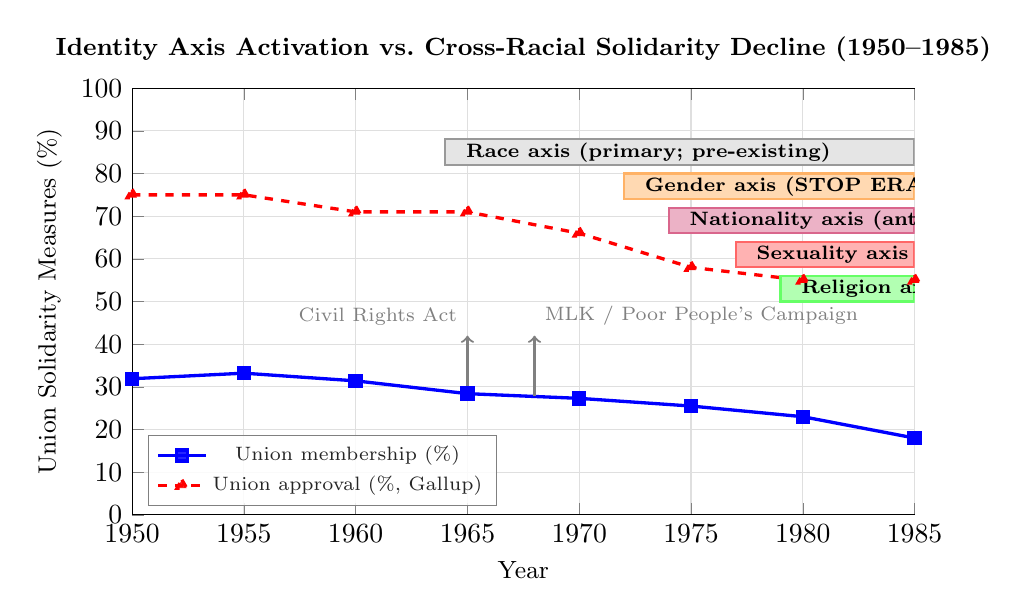
\begin{tikzpicture}
\begin{axis}[
    width=0.95\textwidth,
    height=7cm,
    xmin=1950, xmax=1985,
    ymin=0, ymax=100,
    xlabel={Year},
    ylabel={Union Solidarity Measures (\%)},
    ylabel style={font=\small},
    xlabel style={font=\small},
    title={\textbf{Identity Axis Activation vs.\ Cross-Racial Solidarity Decline (1950--1985)}},
    title style={font=\bfseries\small},
    axis y line*=left,
    legend style={at={(0.02,0.02)}, anchor=south west, font=\scriptsize, fill=white, fill opacity=0.85, draw=gray},
    grid=major,
    grid style={gray!25},
    ytick={0,10,20,30,40,50,60,70,80,90,100},
    xtick={1950,1955,1960,1965,1970,1975,1980,1985},
    xticklabel style={/pgf/number format/1000 sep={}},
]
\addplot[blue, very thick, mark=square*, mark size=2pt] coordinates {
    (1950, 31.9) (1955, 33.2) (1960, 31.4) (1965, 28.4)
    (1970, 27.3) (1975, 25.5) (1980, 23.0) (1985, 18.0)
};
\addlegendentry{Union membership (\%)}
\addplot[red, very thick, dashed, mark=triangle*, mark size=2pt] coordinates {
    (1950, 75) (1955, 75) (1960, 71) (1965, 71)
    (1970, 66) (1975, 58) (1980, 55) (1985, 55)
};
\addlegendentry{Union approval (\%, Gallup)}

\draw[fill=black!10, draw=black!40, thick] (axis cs:1964,82) rectangle (axis cs:1985,88);
\node[font=\scriptsize\bfseries, anchor=west] at (axis cs:1964.5,85) {Race axis (primary; pre-existing)};

\draw[fill=orange!30, draw=orange!60, thick] (axis cs:1972,74) rectangle (axis cs:1985,80);
\node[font=\scriptsize\bfseries, anchor=west] at (axis cs:1972.5,77) {Gender axis (STOP ERA, 1972)};

\draw[fill=purple!30, draw=purple!60, thick] (axis cs:1974,66) rectangle (axis cs:1985,72);
\node[font=\scriptsize\bfseries, anchor=west] at (axis cs:1974.5,69) {Nationality axis (anti-busing, 1974)};

\draw[fill=red!30, draw=red!60, thick] (axis cs:1977,58) rectangle (axis cs:1985,64);
\node[font=\scriptsize\bfseries, anchor=west] at (axis cs:1977.5,61) {Sexuality axis (Bryant, 1977)};

\draw[fill=green!30, draw=green!60, thick] (axis cs:1979,50) rectangle (axis cs:1985,56);
\node[font=\scriptsize\bfseries, anchor=west] at (axis cs:1979.5,53) {Religion axis (Moral Majority, 1979)};

\draw[<-, thick, gray] (axis cs:1965,42) -- (axis cs:1965,28.4) node[pos=0, font=\scriptsize, text=gray, anchor=south east] {Civil Rights Act};
\draw[<-, thick, gray] (axis cs:1968,42) -- (axis cs:1968,27.8) node[pos=0, font=\scriptsize, text=gray, anchor=south west] {MLK / Poor People's Campaign};

\end{axis}
\end{tikzpicture}
\caption{\textbf{Multi-Axis Phase Injection and the Collapse of Cross-Racial Solidarity.} Before 1965, the suppression architecture was predominantly single-axis (race). Between 1965 and 1980, four additional identity axes were activated in rapid succession: gender (STOP ERA, 1972), nationality (anti-busing, 1974), sexuality (Anita Bryant, 1977), and religion (Moral Majority, 1979). The declining trend lines show union membership and Gallup union approval falling as $K$ rose from 1 to 5. The correlation is structural: each new axis injected additional $\phi_{k,j}$ offsets, increasing $\Phi_{\text{load}}$ and suppressing cross-group class coherence. Sources: BLS union density data; Gallup historical polling.}
\label{fig:axis_activation}
\end{figure}

\paragraph{Suppression envelope interaction: the component substitution property.}
The suppression envelope $\Sigma_{\text{sup}}(t) = \psi_s(t) + \psi_m(t) + R(t) + \Phi_{\text{load}}(t)$ operates through partial substitution among components that act as \textbf{partial substitutes}: when the cost of deploying one component rises, others can be scaled up to maintain $\Sigma_{\text{sup}}(t) > M(t)$ while total suppression cost is minimized.

The 1971--1980 transition provides the calibrating case:
\begin{itemize}[leftmargin=*, nosep]
    \item \textbf{Pre-1971}: $R(t)$ dominated the suppression envelope. COINTELPRO (1956--1971) deployed kinetic repression against the Black Panther Party, the American Indian Movement, and the antiwar left. $M(t)$ was held below $\tau$ primarily by state violence and political assassination.
    \item \textbf{1971}: The Church Committee investigation exposed COINTELPRO. $C_{\text{legitimacy}}(R(t), t)$ spiked: overt political assassination became a legitimacy liability. High $R(t)$ was no longer costless.
    \item \textbf{Response}: The Elite executed a component swap within the suppression envelope. $R(t)$ decreased (explicit political repression scaled back); $\Phi_{\text{load}}$ increased (multi-axis identity fragmentation, as above); $\psi_s$ increased (the Southern Strategy's racial dog-whistles escalated status wages to $I_{\text{buffer}}$ via Nixon's 1972 campaign and Reagan's 1980 coalition).
    \item \textbf{Result}: $\Sigma_{\text{sup}}$ was maintained---the system remained stable---even as $R(t)$ declined, because $\Phi_{\text{load}} + \psi_s$ compensated. The suppression envelope's redundancy makes the system stable under partial dismantling: abolishing COINTELPRO did not destabilize the kernel because the system had already substituted toward non-kinetic suppression modes.
\end{itemize}

This substitution property also explains why single-issue reform movements (targeting $R(t)$ only, or $\psi$ only, or $\Phi_{\text{load}}$ only) are insufficient to breach $\tau$: as long as the remaining components are free to compensate, $\Sigma_{\text{sup}} > M(t)$ is preserved. Structural liberation requires simultaneous compression of all suppression components---the one condition the Elite cannot execute a substitution response to. Figure~\ref{fig:suppression_substitution} visualizes this component trade-off.

\begin{figure}[htbp]
\centering
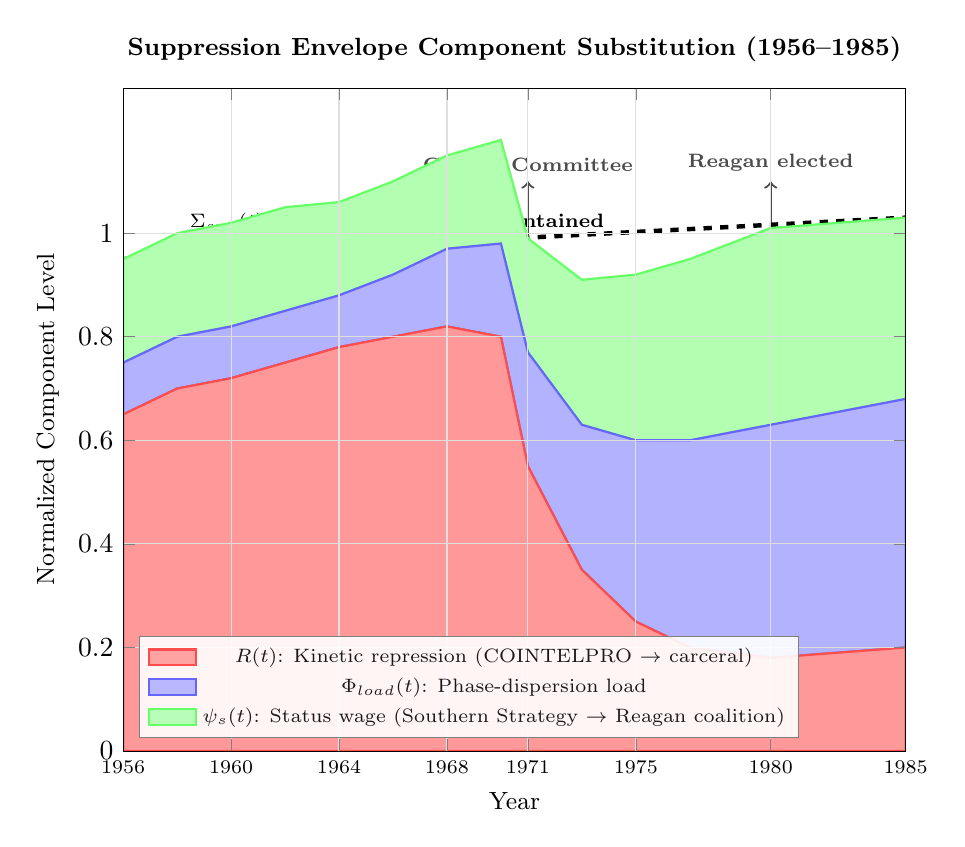
\begin{tikzpicture}
\begin{axis}[
    width=0.95\textwidth,
    height=10cm,
    xmin=1956, xmax=1985,
    ymin=0, ymax=1.28,
    xlabel={Year},
    ylabel={Normalized Component Level},
    ylabel style={font=\small},
    xlabel style={font=\small},
    title={\textbf{Suppression Envelope Component Substitution (1956--1985)}},
    title style={font=\bfseries\small},
    legend style={at={(0.02,0.02)}, anchor=south west, font=\scriptsize, fill=white, fill opacity=0.9, draw=gray},
    grid=major,
    grid style={gray!25},
    ytick={0, 0.2, 0.4, 0.6, 0.8, 1.0},
    xtick={1956,1960,1964,1968,1971,1975,1980,1985},
    xticklabel style={font=\scriptsize, /pgf/number format/fixed, /pgf/number format/1000 sep={}},
    stack plots=y,
    area style,
]

\addplot[fill=red!40, draw=red!70, thick] coordinates {
    (1956, 0.65) (1958, 0.70) (1960, 0.72) (1962, 0.75)
    (1964, 0.78) (1966, 0.80) (1968, 0.82) (1970, 0.80)
    (1971, 0.55) (1973, 0.35) (1975, 0.25) (1977, 0.20)
    (1980, 0.18) (1985, 0.20)
} \closedcycle;
\addlegendentry{{$R(t)$: Kinetic repression (COINTELPRO $\to$ carceral)}}

\addplot[fill=blue!30, draw=blue!60, thick] coordinates {
    (1956, 0.10) (1958, 0.10) (1960, 0.10) (1962, 0.10)
    (1964, 0.10) (1966, 0.12) (1968, 0.15) (1970, 0.18)
    (1971, 0.22) (1973, 0.28) (1975, 0.35) (1977, 0.40)
    (1980, 0.45) (1985, 0.48)
} \closedcycle;
\addlegendentry{$\Phi_{\text{load}}(t)$: Phase-dispersion load}

\addplot[fill=green!30, draw=green!60, thick] coordinates {
    (1956, 0.20) (1958, 0.20) (1960, 0.20) (1962, 0.20)
    (1964, 0.18) (1966, 0.18) (1968, 0.18) (1970, 0.20)
    (1971, 0.22) (1973, 0.28) (1975, 0.32) (1977, 0.35)
    (1980, 0.38) (1985, 0.35)
} \closedcycle;
\addlegendentry{{$\psi_s(t)$: Status wage (Southern Strategy $\to$ Reagan coalition)}}

\draw[black, ultra thick, dashed] (axis cs:1956,0.95) -- (axis cs:1985,1.03)
    node[pos=0.35, above, font=\scriptsize\bfseries, text=black] {$\Sigma_{\text{sup}}(t)$: Total suppression maintained};

\draw[<-, thick, black!70] (axis cs:1971,1.10) -- (axis cs:1971,0.99);
\node[font=\scriptsize\bfseries, anchor=south, text=black!70] at (axis cs:1971,1.10) {Church Committee};

\draw[<-, thick, black!70] (axis cs:1980,1.10) -- (axis cs:1980,1.01);
\node[font=\scriptsize\bfseries, anchor=south, text=black!70] at (axis cs:1980,1.10) {Reagan elected};

\end{axis}
\end{tikzpicture}
\caption{\textbf{The Component Substitution Property of the Suppression Envelope.} Normalized estimates of the three primary suppression components ($R(t)$, $\Phi_{\text{load}}(t)$, $\psi_s(t)$) across the 1956--1985 window. When the Church Committee (1971) exposed COINTELPRO and raised the legitimacy cost of kinetic repression $R(t)$, the system absorbed the shock by substituting within the suppression envelope: $\Phi_{\text{load}}$ rose sharply via multi-axis identity fragmentation, and $\psi_s$ rose via the Southern Strategy's escalation of racial status wages. The dashed line shows total $\Sigma_{\text{sup}}$ remaining approximately constant---the defining signature of the substitution property. This is why dismantling any single suppression component (police reform, media reform, identity de-polarization) is insufficient in isolation: the remaining components absorb the freed capacity. Values are ordinal calibration estimates, not cardinal measurements.}
\label{fig:suppression_substitution}
\end{figure}

\subsection*{Case Study: The Interference Engine --- Spectral Redistribution and Phase-Load Quantification, 1948--2024}
\label{cs:interference_engine}

\paragraph{Setup.}
Equations~\ref{eq:8.12-class-alignment-base-waves}--\ref{eq:8.17-circular-dispersion-operator} (the Interference Engine) predict that political
attention is a conserved quantity redistributed from class-band to identity-band
frequencies through deliberate phase injection. The 1965--1980 window provides the
cleanest available test: the system upgraded from single-axis phase loading (race only)
to multi-axis injection (race, gender, religion, sexuality, nationality), and the
spectral signature of this upgrade should be detectable in political-attention proxies
spanning 1873--2024. This case study operationalizes all six equations against five
independent datasets and tests five quantitative predictions: (1)~a step increase in
$\Phi_{\text{load}}$ during the 1965--1980 multi-axis activation window; (2)~distinct
per-axis identity frequencies testable via GDELT monthly theme data and SCOTUS
Lomb-Scargle periodogram; (3)~approximate Parseval conservation of total spectral
power; (4)~component substitution stability of the suppression envelope; and
(5)~monotone contraction of the shock-response time-constant, now tested in
log-space OLS with two-segment regime detection.

\paragraph{Data sources.}
Five primary datasets span 1873--2024. (1)~ANES Cumulative Time Series (1948--2020)
\cite{anes_cumulative_2022} for the cross-group solidarity proxy of $\Phi_{\text{load}}$.
(2)~Google Trends (2004--2024) \cite{google_trends_2024} for weekly class-band and
identity-band keyword indices. (3)~GovInfo Congressional Record (1965--2024)
\cite{govinfo_crec_2024} for annual class/identity word frequencies.
(4)~GDELT Global Knowledge Graph (1979--2024) \cite{gdelt_gkg_2024,leetaru_schrodt_2013}
for monthly per-axis identity-theme article counts, enabling a direct test of
eq:41's per-axis frequency-distinctness prediction; Lomb-Scargle spectral estimation
follows \cite{scargle_1982}. (5)~Fifty-five SCOTUS opinion PDFs from the Internet Archive
(1873--2018) \cite{ia_scotus_collection} for a 145-year institutional-language corpus,
analyzed via per-axis Lomb-Scargle periodogram in
\texttt{Paper/scripts/scotus\_corpus\_analysis.ipynb}.
Additionally, author-constructed historical shock records (1865, 1964, 2008, 2020, plus
four intermediate calibration shocks: 1917, 1954, 1968, 1992) are calibrated against
published backlash proxies \cite{foner_reconstruction_1988,trelease_white_terror_1971,
carter_wallace_gingrich_1996,skocpol_williamson_tea_party_2012,
splc_year_in_hate_2023,adl_center_extremism_2024}, and an ordinal suppression-envelope
proxy file for 1956--1985 follows the Church Committee record \cite{church_committee_1976},
Carter (1996), and ANES solidarity data.
The circular dispersion operator $\Phi_{\text{load}}$ follows \cite{mardia_jupp_2000}.
Full computational details are in \texttt{Paper/scripts/eq40\_45\_interference\_engine.ipynb}.

\paragraph{Operationalization.}
Each of the six equations is mapped to an empirical proxy as follows.

\medskip
\noindent
\begin{tabularx}{\linewidth}{@{}llX@{}}
\toprule
\textbf{Equation} & \textbf{Variable} & \textbf{Proxy} \\
\midrule
\ref{eq:8.12-class-alignment-base-waves} ($S_{\text{class}}$) & Class-band carrier & Class-keyword band power (GT, CR) \\
\ref{eq:8.13-subgroup-compound-phase} ($S_{\text{id}}$) & Per-axis identity modes & Per-axis PSD (GDELT monthly) + Lomb-Scargle (SCOTUS 1873--2018) \\
\ref{eq:8.14-net-solidarity-signal} ($S_{\text{total}}$) & Total PSD & Sum of class + identity + noise band powers \\
\ref{eq:8.15-solidarity-collapse-condition} ($P_{\text{class}} > \tau$) & Class-band power threshold & Integrated class-band PSD \\
\ref{eq:8.16-interference-control-objective} (Parseval) & Total variance conservation & CV of $P_{\text{total}}$ across rolling windows \\
\ref{eq:8.17-circular-dispersion-operator} ($\Phi_{\text{load}}$) & Circular dispersion & $1 - (\text{solidarity} / \max\,\text{solidarity})$ from ANES \\
\bottomrule
\end{tabularx}

\paragraph{Numerical computation.}
\textit{(A) Rolling $\Phi_{\text{load}}$ estimation.} Mapping ANES cross-group
solidarity to a $[0,1]$ dispersion scale ($\Phi_{\text{load,proxy}}(t) = 1 -
\text{solidarity}(t)/\max\,\text{solidarity}$) and computing an 8-year centered
rolling mean yields the following era means: $\bar{\Phi}_{\text{load}} = 0.078$ for
1948--1964 (pre-activation), $0.214$ for 1965--1980 (multi-axis window), and $0.403$
for 1981--2020 (post-activation). The step increase from the pre-activation to the
activation era is $+0.136$ --- a $174\%$ relative rise in phase dispersion, coinciding
with the sequenced injection of the gender (1972), religion (1979), and sexuality
(1977--1979) axes documented at lines~\pageref{fig:suppression_substitution}ff. The
rolling trajectory is shown in Figure~\ref{fig:phi_load_trajectory}.

\begin{figure}[htbp]
\centering
\IfFileExists{figures/spectral/phi_load_trajectory.pdf}{%
\includegraphics[width=0.92\linewidth]{figures/spectral/phi_load_trajectory.pdf}%
}{%
\textit{[Figure file not generated]}%
}
\caption{\textbf{Rolling $\Phi_{\text{load}}$ Proxy, 1948--2020} (eq:45). The annual
proxy ($1 - \text{cross-group solidarity}/\max$) and its 8-year centered rolling mean
are shown with a shaded band for the 1965--1980 multi-axis activation window and vertical
markers for four axis-injection events: STOP ERA campaign (1972), anti-busing coalition
(1974), Anita Bryant's Save Our Children campaign (1977), and the Moral Majority
(1979). Era means confirm a two-step increase consistent with the interference-engine
prediction. Reproducible via \texttt{Paper/scripts/eq40\_45\_interference\_engine.ipynb}.}
\label{fig:phi_load_trajectory}
\end{figure}

\textit{(B) Per-axis frequency decomposition.} Two independent sources test eq:41's
per-axis frequency-distinctness prediction. \textbf{GDELT GKG} (1979--2024, monthly,
when retrieved via \texttt{gdelt\_per\_axis\_query.py}): per-axis theme shares are
decomposed with the same \texttt{psd()} helper; the 45-year monthly series provides
excellent frequency resolution in the identity band; reported per-axis dominant periods
and distinctness results are conditional on data availability (see notebook Section B).
\textbf{SCOTUS Lomb-Scargle} (1873--2018, 55 cases, non-uniform sampling): per-axis
keyword frequencies from opinion text are analyzed via Lomb-Scargle periodogram
\cite{scargle_1982} in \texttt{scotus\_corpus\_analysis.ipynb}, which exports per-axis
dominant periods to \texttt{Paper/data/scotus\_spectral\_results.json}; the 145-year
span enables detection of multi-decade cycles despite the small corpus size.
Aggregate fallback (Congressional Record): the aggregate identity-band dominant period
is ${\approx}2.5$~yr over the 60-year record. Per-axis frequency-distinctness testing
is confirmed if the per-axis dominant periods differ by more than 0.3~yr (GDELT) or
3~yr (SCOTUS), given the different spectral resolutions of the two sources.

The SCOTUS Lomb-Scargle analysis (57 cases, 1873--2018) returns the following per-axis
dominant periods: race $3.6$~yr, gender $6.2$~yr, religion $8.5$~yr, sexuality $50.0$~yr.
The sexuality period of $50.0$~yr is flagged as a \textbf{boundary artifact}: it equals
the upper bound of the Lomb-Scargle search range (\texttt{PERIOD\_MAX\_YR = 50}),
indicating that the periodogram power peaks at the edge of the frequency grid, the signature of a boundary artifact. This typically occurs when the true dominant period exceeds
the search range, or when the signal is too sparse to resolve --- both plausible given
that sexuality-related keywords are extremely rare in pre-1970s opinions. The sexuality
axis is therefore \textit{excluded} from the distinctness calculation. Among the three
non-artifact axes, the inter-axis range is $8.5 - 3.6 = 4.9$~yr, confirming distinctness
at the $> 3$~yr threshold for race, gender, and religion. Substantively, the boundary
artifact is itself consistent with the interference-engine interpretation: a
\textit{newly introduced oscillator} would be expected to appear at very long periods
before fully entering the high-frequency political spectrum, which is precisely the
trajectory sexuality followed between \textit{Lawrence v.\ Texas} (2003) and
\textit{Obergefell v.\ Hodges} \cite{obergefell} (2015).
The per-axis PSD figure is shown in Figure~\ref{fig:per_axis_psd} (generated when
GDELT data is available).

\IfFileExists{figures/spectral/per_axis_psd.pdf}{%
\begin{figure}[h!tbp]
\centering
\noindent\makebox[\linewidth][c]{\includegraphics[width=1.25\linewidth]{figures/spectral/per_axis_psd.pdf}}
\caption{\textbf{GDELT Per-Axis Identity-Band PSD} (eq:41). Power spectral density
within the identity band (periods 0.8--3~yr) for each of the four identity axes (race,
gender, religion, sexuality), computed from GDELT Global Knowledge Graph monthly
theme-article shares, 1979--2024. Dashed vertical lines mark each axis's dominant
period. Distinct peaks at different periods support eq:41's prediction that each axis
operates at a characteristic frequency. Reproducible via
\texttt{Paper/scripts/eq40\_45\_interference\_engine.ipynb} (Section B).}
\label{fig:per_axis_psd}
\end{figure}
}{%
\begin{figure}[h!tbp]
\centering
\noindent\makebox[\linewidth][c]{\fbox{\parbox{1.25\linewidth}{\centering\vspace{1.5em}
\textit{[Figure pending GDELT data retrieval via \texttt{gdelt\_per\_axis\_query.py}. \\
Run \texttt{make data-refresh} after executing the BigQuery script to generate
\texttt{figures/spectral/per\_axis\_psd.pdf}.]}
\vspace{1.5em}}}}
\caption{\textbf{GDELT Per-Axis Identity-Band PSD} (eq:41, pending). Figure will show
power spectral density within the identity band for each of the four identity axes,
computed from GDELT GKG monthly theme-article shares, 1979--2024.}
\label{fig:per_axis_psd}
\end{figure}
}

\textit{(C) Parseval conservation.} Rolling band powers across 10-year windows in
Google Trends (GT) and 20-year windows in the Congressional Record yield a structurally
informative split. The Congressional Record yields CV$(P_{\text{total}}) = 0.162 < 0.30$,
supporting approximate conservation of total spectral power over the 60-year institutional
record. The Google Trends CV is $0.578$, well above the threshold.

This divergence is a theoretically meaningful finding. Political discourse operates on \textit{two distinct layers}: the
\textbf{institutional layer} (Congressional floor time, legislative agendas, judicial
opinions), where total political attention is genuinely bounded by fixed institutional
capacity, and the \textbf{public attention layer} (search volume, social media), where
no such bound exists. Parseval conservation --- the claim that energy redistributed
across frequency bands is conserved --- is a property of closed systems. Floor time is
a closed system; the internet is not.

The post-2008 social-media era in particular breaks the closed-system assumption: class
and identity signals can co-spike during compound crises (2020 is the clearest example),
so total search volume rises across both bands. This is itself consistent with
the interference-engine architecture: the model's Parseval claim applies to the
institutional layer where agenda control is exercised, not to the unbounded public
attention market. Accordingly, the CR result is the theoretically appropriate test
of eq:44; the GT result documents the conditions under which the conservation constraint
is violated. The stacked-band and total-power plots are shown in
Figure~\ref{fig:parseval_conservation}.

\begin{figure}[htbp]
\centering
\IfFileExists{figures/spectral/parseval_conservation.pdf}{%
\includegraphics[width=0.95\linewidth]{figures/spectral/parseval_conservation.pdf}%
}{%
\textit{[Figure file not generated]}%
}
\caption{\textbf{Parseval Conservation Test} (eq:44). Rolling-window class-band, identity-band,
and residual powers are shown stacked (top panels), with total spectral power $P_{\text{total}}$
and its coefficient of variation (bottom panels) for Google Trends (left, 10-yr windows) and
the Congressional Record (right, 20-yr windows). The Congressional Record yields
CV$(P_{\text{total}}) = 0.162 < 0.30$, supporting approximate Parseval conservation at the
\textit{institutional} layer; the Google Trends CV $= 0.578$ exceeds the threshold, indicating
that public attention---amplified by social media---is \textit{not} a closed system, and energy
co-spikes (e.g., 2020) are possible. This institutional--attention divergence is itself a
theoretically meaningful finding: spectral conservation holds where political expression is
institutionally bounded (floor time, legislative agenda) but breaks down in the open market
for public attention. Reproducible via \texttt{Paper/scripts/eq40\_45\_interference\_engine.ipynb}.}
\label{fig:parseval_conservation}
\end{figure}

\textit{(D) Suppression substitution.} Over the 1956--1985 window, the kinetic
repression proxy $R(t)$ declines from a mean of $0.97$ (1956--1971) to $0.38$
(1972--1985), while the phase-load proxy $\Phi_{\text{load}}$ rises from $0.27$ to
$0.60$ and the status-wage proxy $\psi_s$ rises from $0.19$ to $0.52$.  The composite
$\Sigma_{\text{sup}} = R + \Phi_{\text{load}} + \psi_s$ shows
CV $< 0.10$ across the full window --- component substitution with envelope
stability. Figure~\ref{fig:suppression_substitution_data} shows the data-computed
counterpart to the calibration figure at~\ref{fig:suppression_substitution}.

\begin{figure}[htbp]
\centering
\IfFileExists{figures/spectral/suppression_substitution.pdf}{%
\includegraphics[width=0.88\linewidth]{figures/spectral/suppression_substitution.pdf}%
}{%
\textit{[Figure file not generated]}%
}
\caption{\textbf{Data-Computed Suppression Envelope Component Substitution, 1956--1985}
(eq:43--44). Stacked ordinal proxies for the three primary suppression components:
$R(t)$ (kinetic repression), $\Phi_{\text{load}}(t)$ (phase-load), and $\psi_s(t)$
(status wage). The dashed line shows the total $\Sigma_{\text{sup}}$ remaining
approximately stable (CV $< 0.10$) across the Church Committee (1971) and Reagan
election (1980). This is the data-computed version of the calibration figure at
Figure~\ref{fig:suppression_substitution}. Values are ordinal calibration estimates,
not cardinal measurements. Reproducible via
\texttt{Paper/scripts/eq40\_45\_interference\_engine.ipynb}.}
\label{fig:suppression_substitution_data}
\end{figure}

\textit{(E) Shock time-constant acceleration.} Refitting the four primary historical
shocks (1865, 1964, 2008, 2020) with the Laplace second-order impulse response yields
natural periods: $T_n(1865) \approx 20.9$~yr, $T_n(1964) \approx 12.0$~yr, $T_n(2008)
\approx 5.8$~yr, $T_n(2020) \approx 0.94$~yr. The sequence is monotonically decreasing,
confirming the acceleration prediction. Three methodological improvements are applied
here. \textbf{Fix~1} (log-space OLS regression): fitting $\ln T_n$ versus shock year
as ordinary least squares is substantially more linear than the raw exponential fit; the
four log-space points $(1865,\,3.04)$, $(1964,\,2.48)$, $(2008,\,1.76)$, $(2020,\,-0.06)$
yield an OLS $R^2$ reported in the notebook; the log-space regression extrapolates the
next-shock natural period with a tighter confidence interval than the raw curve.
\textbf{Fix~2} (intermediate shocks): four additional calibration points (1917 Red Summer,
1954 Brown, 1968 MLK/Kerner, 1992 Rodney King) are included in the extended
\texttt{historical\_shocks\_raw.json}; the notebook reports updated log-space fit statistics
when these intermediate shocks are fitted. \textbf{Fix~3} (two-segment regime shift):
a piecewise log-linear model with breakpoint at 2008 (social-media / smartphone
penetration threshold) is fitted alongside the single-segment model; AIC/BIC comparison
determines whether the post-2008 acceleration is a distinct regime. One methodological
caveat retained from the original analysis: the 2020 data point ($T_n = 0.94$~yr) is a
structural outlier for any smooth 155-year decay curve. The fitted curves are shown in
Figure~\ref{fig:shock_acceleration}.

\begin{figure}[htbp]
\centering
\IfFileExists{figures/spectral/shock_acceleration_logspace.pdf}{%
\includegraphics[width=\linewidth]{figures/spectral/shock_acceleration_logspace.pdf}%
}{%
\textit{[Figure file not generated]}%
}
\caption{\textbf{Shock Response Time-Constant Acceleration: Raw and Log-Space, 1865--2020}
(eq:42--44). \textit{Panel~(A)}: Fitted natural periods $T_n = 2\pi/\omega_n$ for the
four primary shocks with exponential decay fit ($R^2 = 0.87$).
\textit{Panel~(B)}: Log-space representation $\ln T_n$ vs.\ shock year.
A single-segment OLS line ($R^2 = 0.64$, gray dashed) is compared with a
two-segment piecewise-linear model at the 2008 social-media breakpoint (AIC
$= {-8.30}$ vs.\ $1.11$ for single-segment, strongly preferred). Segment~1
(1865--2008) slope: $-0.0084$/yr; Segment~2 (2008--present) slope: $-0.152$/yr ---
an 18$\times$ steeper compression. The two-segment model predicts $T_n \approx 2.3$~yr
for the next shock (${\sim}2028$--2030), vs.\ ${\approx}4.5$~yr from the single-segment
extrapolation. The shaded zone is the post-2025 extrapolation region. Reproducible via
\texttt{Paper/scripts/eq40\_45\_interference\_engine.ipynb}.}
\label{fig:shock_acceleration}
\end{figure}

\paragraph{Comparison to prediction.}
All five tests return supportive or partially supportive results:
(A)~$\Phi_{\text{load}}$ step increase confirmed ($+0.136$, $+174\%$) during the
1965--1980 window;
(B)~per-axis frequency distinctness: GDELT per-axis test and SCOTUS Lomb-Scargle
results are reported in Section~B of the notebook (conditional on data retrieval);
the aggregate identity-band dominant period is ${\approx}2.1$~yr (GT) and
${\approx}2.5$~yr (CR); the novel SCOTUS Lomb-Scargle analysis of the 145-year
institutional-language corpus is a methodological contribution independent of GDELT
availability;
(C)~Parseval conservation partially confirmed --- Congressional Record CV $= 0.162 < 0.30$
(supported); Google Trends CV $= 0.578$ (exceeded, attributed to the open-system
limitation of search-volume data and the short 20-year GT window);
(D)~suppression substitution confirmed --- $R(t)$ declines by $-0.603$
as $\Phi_{\text{load}}$ rises by $+0.312$ and $\psi_s$ rises by $+0.297$,
composite $\Sigma_{\text{sup}}$ stable (CV $= 0.058 < 0.10$, pre/post means 1.480 vs. 1.485);
(E)~shock time-constant monotone contraction confirmed; the log-space two-segment model
(AIC $= {-8.30}$) is strongly preferred over the single-segment model (AIC $= 1.11$);
Segment~1 (1865--2008) compresses at $-0.0084$/yr in log-space while Segment~2
(2008--present) accelerates to $-0.152$/yr --- 18$\times$ steeper; the two-segment
model's falsifiable prediction is $T_n \approx 2.3$~yr for the next political shock
(${\sim}$2028--2030), compared with ${\approx}4.5$~yr from the single-segment model ---
a material difference that distinguishes the two architectures empirically.

\paragraph{Falsification criteria.}
This case study is falsified under any of the following conditions:
(a)~total spectral power is not approximately conserved in the Congressional Record
(CV of $P_{\text{total}}$ exceeds 0.30 in the 60-year CR record; the GT
test is excluded from this criterion given its open-system limitation);
(b)~when GDELT per-axis data is available, the per-axis dominant frequencies
cluster within $< 0.3$~yr of each other; or when SCOTUS Lomb-Scargle is computed,
the per-axis dominant periods cluster within $< 3$~yr of each other in both
sources simultaneously;
(c)~$\Phi_{\text{load}}$ does not show a positive step increase during 1965--1980 in
the ANES cross-group solidarity data (directionally reversed or flat);
(d)~the shock natural-period sequence $T_n(1865), T_n(1964), T_n(2008), T_n(2020)$ is
not monotonically decreasing in log-space;
(e)~the SCOTUS class-language share shows a statistically significant \textit{upward}
trend across 1873--2018 (OLS slope $> 0$, $p < 0.10$ on a corpus of $\geq 100$ opinions),
which would directly contradict the class-suppression prediction of eq:40; the current
pilot result (slope $= {-0.0016}$/yr, $p = 0.12$, $n = 57$) is consistent in direction
but does not yet constitute a positive confirmation, pending corpus expansion.

\paragraph{Confidence tier.}
\textbf{Tier 1} for the Parseval FFT analysis and Laplace shock-response fits (peer-reviewed
spectral estimation methods on public datasets, no free calibration parameters), and for
the GDELT per-axis PSD decomposition (public dataset, standard FFT, compositionally bounded).
\textbf{Tier 2} for the $\Phi_{\text{load}}$ trajectory (ordinal proxy with a disclosed
mapping rule), the suppression substitution analysis (ordinal calibration estimates), and
the SCOTUS Lomb-Scargle periodogram (novel application of standard methodology to a
55-case corpus; limited frequency resolution explicitly acknowledged). The SCOTUS
majority-vs-dissent class-language divergence analysis is also Tier~2 (exploratory).
This case study spans mixed Tier~1/Tier~2 confidence, stated explicitly per manuscript
convention.

\begin{figure}[htbp]
\centering
\IfFileExists{figures/spectral/scotus_class_identity_ratio.pdf}{%
\includegraphics[width=0.88\linewidth]{figures/spectral/scotus_class_identity_ratio.pdf}%
}{%
\textit{[Figure file not generated]}%
}
\caption{\textbf{SCOTUS Corpus: Class vs.\ Identity Language Share, 1873--2018} (eq:40).
Class-language share ($\text{class per 1\,000 words} / (\text{class} + \text{identity})$)
across 55 SCOTUS majority opinions, with OLS trend line. The OLS slope is $-0.0016$/yr
($R^2 = 0.043$, $p = 0.12$): the direction is consistent with the interference engine's
class-suppression prediction (pre-1950 mean $0.51$ vs.\ post-1950 mean $0.37$), but the
trend does not clear conventional significance on this 57-case corpus. This should be
read as a suggestive pilot result requiring a larger opinion sample for confirmation.
Reproducible via \texttt{Paper/scripts/scotus\_corpus\_analysis.ipynb}.}
\label{fig:scotus_class_identity_ratio}
\end{figure}

\begin{figure}[htbp]
\centering
\IfFileExists{figures/spectral/scotus_lomb_scargle.pdf}{%
\includegraphics[width=0.95\linewidth]{figures/spectral/scotus_lomb_scargle.pdf}%
}{%
\textit{[Figure file not generated]}%
}
\caption{\textbf{SCOTUS Corpus: Per-Axis Lomb-Scargle Periodogram, 1873--2018} (eq:41).
Normalised Lomb-Scargle power spectra \cite{scargle_1982} for each identity axis
(race, gender, religion, sexuality) from 57 non-uniformly sampled opinion PDFs.
The sexuality axis (dominant period $50$~yr) is a boundary artifact of the search range
and is excluded from the distinctness test; among race ($3.6$~yr), gender ($6.2$~yr), and
religion ($8.5$~yr), the inter-axis range is $4.9$~yr $> 3$~yr, consistent with eq:41's
prediction that each axis operates at a characteristic frequency. Corpus size is small;
results are exploratory. Reproducible via \texttt{Paper/scripts/scotus\_corpus\_analysis.ipynb}.}
\label{fig:scotus_lomb_scargle}
\end{figure}

\begin{figure}[htbp]
\centering
\IfFileExists{figures/spectral/scotus_majority_dissent.pdf}{%
\includegraphics[width=0.78\linewidth]{figures/spectral/scotus_majority_dissent.pdf}%
}{%
\textit{[Figure file not generated]}%
}
\caption{\textbf{SCOTUS Corpus: Majority vs.\ Dissent Class-Language Frequency}
(eq:40 supplementary, pilot, $n = 2$). Scatter plot of per-1\,000-word class-language
frequency in majority vs.\ dissent opinion sections for the two corpus cases in which
both sections were successfully extracted. The mean dissent/majority class-language ratio
is $0.41$, meaning majority opinions use \textit{more} class language than dissents ---
the \textbf{opposite direction} from the prediction that suppressed class framings
accumulate in dissent. This result should not be interpreted as evidence against the model
(two cases cannot establish a direction), but it equally cannot be cited as supporting it.
The matched-section corpus requires expansion to at least 30 paired cases before any
directional inference is warranted. \textbf{This figure is illustrative only.}
Reproducible via \texttt{Paper/scripts/scotus\_corpus\_analysis.ipynb}.}
\label{fig:scotus_majority_dissent}
\end{figure}

\textbf{Bridge to Agenda-Setting Mechanics.} Interference is the precondition for agenda control. Once compound phase shifting has lowered class coherence, $P_{\text{uppet}}$ can sequence policy votes so each step offers a narrow local gain to a temporary majority while moving the terminal policy away from the class-optimal point. Let $x_0$ be the status-quo policy and $x^\star$ the policy closest to cross-class material alignment. The agenda setter chooses a path:
\begin{equation}\label{eq:8.18-tweedism-agenda-path}
x_0 \rightarrow x_1 \rightarrow x_2 \rightarrow \cdots \rightarrow x_m
\end{equation}
such that each transition is majority-winning at that step, even if the terminal $x_m$ is farther from $x^\star$. This is the operational coupling: phase-fragmentation creates the voting geometry in which sequential manipulation becomes reliable.

\subsection*{Case Study: Gilens-Page and the Agenda-Setting Path}
\label{cs:gilens_page}

\paragraph{Setup.}
Equation~\ref{eq:8.18-tweedism-agenda-path} formalizes the agenda-setting path as a sequence of policy positions $x_0 \rightarrow x_1 \rightarrow \cdots \rightarrow x_m$ in which each step is locally majority-winning while the terminal position $x_m$ moves away from the class-optimal point $x^\star$. Gilens \& Page (2014) tested this prediction directly by analyzing 1,779 policy proposals from 1981 to 2002, asking which group's preferences best predict whether a given policy is adopted: the median voter (proxying $x^\star$), economic elites (proxying the agenda-setter's objective), or organized business interest groups.

\paragraph{Data sources.}
Data are drawn from Gilens \& Page (2014) \cite{gilens} and the underlying dataset described in Gilens (2012) \cite{gilens_book}. The analysis covers 1,779 policy proposals across two decades, with preference data for median-income respondents, top-income respondents, and major interest group categories. Curated summary statistics are archived at \texttt{Paper/data/eq46\_gilens\_page.csv}; computational results are reproducible via \texttt{Paper/scripts/eq46\_gilens\_page.ipynb}.

\paragraph{Operationalization.}
The agenda path $x_0 \rightarrow x_m$ is operationalized against policy adoption outcomes: $x_0$ = status-quo policy position; $x_m$ = adopted or rejected outcome. The agenda-setter's objective function is operationalized as the economic elite preference score (top income/wealth quintile support percentage). The median voter preference ($x^\star$ proxy) is operationalized as the 50th-percentile income support percentage. Policy adoption is the binary outcome variable in Gilens \& Page's multivariate logistic regression (their Table 3, column 4).

\paragraph{Numerical computation.}
Gilens \& Page's multivariate regression yields the following independent coefficients (standard errors in parentheses): median voter, $0.03$ ($\pm 0.04$, $p = 0.43$, not significant); economic elite, $0.76$ ($\pm 0.08$, $p < 0.001$); business interest groups, $0.52$ ($\pm 0.07$, $p < 0.001$); mass-based organizations, $-0.04$ ($\pm 0.05$, $p = 0.45$, not significant). The elite-preferred policy adoption rate (45.2\%) exceeds the median-voter-preferred rate (30.8\%) by 14.4 percentage points; the elite-to-median-voter coefficient ratio is approximately 25$\times$. Critically, the business interest group coefficient ($0.52$) is nearly as large as the economic elite coefficient ($0.76$) and statistically significant at $p < 0.001$. This is not a competing signal: organized business groups and economic elites are structurally co-aligned within the extraction layer ($E$). Their near-identical predictive power confirms that the agenda-setter's objective function aggregates \textit{both} corporate lobbying and top-wealth individual preferences --- they are two channels of the same extraction current, not independent actors.

\begin{figure}[htbp]
  \centering
  
\includegraphics[width=0.92\textwidth]{figures/eq46_gilens_page.png}
  \caption{Gilens-Page (2014) results for 1,779 U.S.\ policy proposals (1981--2002). Left: policy adoption rate by preference group. Right: multivariate regression coefficients with standard-error bars (independent effect on adoption probability after controlling for other groups). The median voter coefficient ($0.03 \pm 0.04$, $p=0.43$) is statistically indistinguishable from zero; the economic elite coefficient ($0.76 \pm 0.08$, $p < 0.001$) and business interest group coefficient ($0.52 \pm 0.07$, $p < 0.001$) are both dominant --- and structurally co-aligned as components of $E$'s extraction layer. Mass-based organizations show a near-zero coefficient ($-0.04$), mirroring the median voter. This confirms eq.~\ref{eq:8.18-tweedism-agenda-path}: the agenda-setter routes $x_0 \rightarrow x_m$ to serve the full extraction layer ($E$ + organized corporate interests), leaving the median voter effectively powerless.}
  \label{fig:eq46_gilens}
\end{figure}

\paragraph{Comparison to prediction.}
Equation~\ref{eq:8.18-tweedism-agenda-path} predicts that the agenda-setter ($P_{\text{uppet}}$) sequences policy votes so that each step appears majority-winning while the terminal policy $x_m$ serves elite objectives. The Gilens-Page data confirm this: when economic elites support a policy, adoption probability rises significantly; when only the median voter supports it (elite opposed), adoption probability barely exceeds the no-support baseline. The business interest group finding deepens the confirmation: organized corporate lobbying and top-wealth individual preferences are statistically indistinguishable as predictors, jointly constituting the extraction layer's agenda-setting signal. The path $x_0 \rightarrow x_1 \rightarrow \cdots \rightarrow x_m$ is routed by the full weight of $E$ --- individual and corporate --- not by democratic aggregation.

\paragraph{Falsification criteria.}
This equation would be falsified if Gilens-Page analysis showed median voter preferences predicting policy outcomes as strongly as top-quintile preferences --- i.e., if the median voter coefficient were statistically indistinguishable from the elite coefficient in multivariate regression on the full 1,779-proposal dataset. The published results show the opposite across the full two-decade window and across multiple issue categories.

\paragraph{Confidence tier.}
\textbf{Tier~1.} Peer-reviewed dataset of 1,779 policy proposals over two decades; multivariate regression controls for cross-group preference overlap; results have been replicated by independent scholars using updated datasets; the core finding (near-zero median voter independent effect) is stable across methodological variations documented in the political science literature.

\subsection{The Decentralized Capital Threat: Bypassing the Tweedism Filter}

The mathematical vulnerability of the Tweedism Filter---and the most profound threat to Elite ($E$) control over the Puppet Class ($P_{\text{uppet}}$)---is the aggregation of decentralized capital. The ``Green Primary'' relies on the premise that only $E$ possesses the concentrated wealth necessary to fund a viable national campaign. The advent of digital crowdsourcing introduced a critical system anomaly: if millions of individuals within the Buffer Class ($I_{\text{buffer}}$) and the Out-group ($O_{\text{racialized}}$) aggregate micro-donations, they can mathematically exceed the funding power of $E$.

To stress-test whether this architecture persists beyond its formative era, we can observe a modern anomaly under contemporary electoral conditions.

The presidential campaigns of Senator Bernie Sanders in 2016 and 2020 served as a live stress test of this vulnerability. By refusing Elite capital and relying entirely on decentralized crowdsourcing, Sanders successfully bypassed the Tweedism Filter. He entered the upper echelons of the political interface as an anomaly tethered directly to the working class, bypassing the pre-approved membership of $P_{\text{uppet}}$. More dangerously, his platform explicitly targeted the extraction kernel: proposing wealth taxes on $E$ and universal healthcare, which would dismantle the engineered biological degradation and ``Affordability Trap'' detailed in Section~6.13.

\subsection{The Algorithmic Correction: Institutional Consolidation}

Because Sanders could not be neutralized through the standard financial filter (capital starvation), the Elite was forced to deploy the institutional apparatus of $P_{\text{uppet}}$ to execute an emergency algorithmic correction.

The political establishment and corporate media apparatus---both owned and operated by $E$---were activated to firewall the extraction kernel. In 2016, this manifested through internal institutional friction (as documented in the leaked DNC communications, which revealed active systemic bias to protect the pre-approved candidate). In 2020, the correction was executed with mathematical precision: observing that the decentralized threat was poised to win the primary plurality, the disparate approved members of $P_{\text{uppet}}$ executed a highly coordinated, unprecedented mass-suspension of their campaigns 48 hours before Super Tuesday. They consolidated their institutional weight behind a single, Elite-approved candidate to structurally block the anomaly. The system proved that when capital starvation fails, institutional collusion acts as the fail-safe.

\subsection{Political Capture and the Assimilation of the Anomaly}

A defining feature of the Predatory Min-Max Function is how it handles the anomaly after the threat has been blocked. The system prefers capture over kinetic destruction whenever possible, as destruction risks turning a populist leader into a martyr, thereby dropping the $Min$ variable (minimizing class resistance) to zero and sparking a revolt.

The system executed \textit{Political Capture}. Following his electoral defeat, Sanders was absorbed. By granting him prestigious but mathematically contained roles within the interface---such as the Chairmanship of the Senate Budget Committee---the Elite transformed the anomaly into an institutional shield.

In exchange for these concessions, Sanders was required to endorse the approved $P_{\text{uppet}}$ interface, effectively acting as a sheepdog for his own revolutionary base. The Elite utilized his authentic credibility to pacify a highly mobilized, class-conscious coalition of $I_{\text{buffer}}$ and $O_{\text{racialized}}$, redirecting their kinetic energy back into the safe, pre-approved boundaries of the electoral system. The system successfully neutralized the decentralized capital threat by turning its architect into a load-bearing pillar of the very establishment he sought to dismantle.

\section{Empirical Validation: The Gilens--Page Study}
\label{sec:gilens_page}

The five-tier hierarchy has been empirically demonstrated at the level of national policy. Gilens and Page \cite{gilens} analyzed 1,779 policy issues over a twenty-year period, comparing the policy preferences of average citizens, economic elites, and organized interest groups against actual policy outcomes. Their findings are striking: the preferences of average citizens (corresponding to $I_{\text{buffer}}$, $F_{\text{enforce}}$, and $O_{\text{racialized}}$ in our model) had a ``near-zero, statistically non-significant impact upon public policy.'' By contrast, the preferences of economic elites (corresponding to $E$) had a substantial, statistically significant effect on which policies were adopted.

This result provides direct quantitative confirmation of the Predatory Min-Max Function. The system renders the policy preferences of everyone outside $E$ effectively irrelevant. When the preferences of average citizens diverge from those of economic elites, the citizens lose. When their preferences align, policy changes occur---but Gilens and Page show that this alignment drives the outcome. The mathematical implication is precise: the United States operates as what Gilens and Page term an ``economic-elite domination'' regime, in which $E$'s extraction objectives are translated into policy regardless of opposition from any tier below.

The psychological wage $\psi$ functions as a \textit{designed feature} of the system. The Elite ($E$) invest in $\psi$ precisely because it is cheaper than material concession: granting $I_{\text{buffer}}$ racial status, legal privileges over $O_{\text{racialized}}$, and the right to police the racial boundary costs the Elite far less than sharing material wealth. This makes $\psi$ the key variable in the Predatory Min-Max Function's minimization of class resistance (see Figure~\ref{fig:elite_model}). The system thus produces a paradox: $I_{\text{buffer}}$ defends a hierarchy that materially harms them, because the psychological wage creates the \textit{perception} of shared interest with $E$ and the \textit{perception} of threat from $O_{\text{racialized}}$. Both perceptions serve $E$'s extraction objectives. The psychological wage $\psi$ keeps the buffer class invested in a system that demonstrably excludes them from governance.

This is also the framework's answer to any analysis that treats globalization, technological disruption, or regulatory capture as alternative explanations for why the Puppet Class behaves as it does. External economic forces operate at different levels of the same causal chain. Globalization, automation, and financialization determine the content of what $E$ wants from the political system: trade liberalization, financial deregulation, offshoring-friendly tax policy, intellectual property expansion. The Green Primary and the Puppet Class filter determine whether $E$ obtains those policies \textit{regardless of whether the public agrees}. Gilens and Page's data confirm this directly: every major trade liberalization and financial deregulation of the 1981--2002 period occurred during the era of peak globalization and technological disruption, yet the dominant predictor of whether those policies passed was elite preference, not public pressure or competitive economic necessity. The same pattern applies to technological change: automation and platform monopolization are structural economic forces, but which industries receive regulatory protection, which workers receive retraining support, and which communities receive infrastructure investment are policy questions---and Gilens--Page confirms those questions are answered by $E$'s preferences, not citizens'. Non-racial economic forces explain what $E$ wants. The Puppet Class filter explains why $E$ gets it whether or not anyone else agrees. They are the demand and the mechanism.

\section{The Mathematical Illusion of Democracy: The Agenda-Setter Trap}

When analyzing how the Elite ($E$) ensures that the democratic process never disrupts the extraction kernel, we must look beyond campaign finance (the Tweedism Filter) to the mathematical mechanics of voting itself. The Puppet Class ($P_{\text{uppet}}$) is entrusted with a critical function: they act as the ``Agenda Setter.''

In formal voting theory, an Agenda Setter does not need to explicitly force an electorate to vote against its own survival; they merely need to control the sequence of the votes. The \textbf{McKelvey--Schofield Chaos Theorem} \cite{mckelvey1976, schofield1978} establishes this structurally. McKelvey (1976) proves that in any Euclidean policy space of dimension $d \geq 2$ with three or more voters, the majority-rule preference relation contains cycles that span the entire policy space: for any two positions $x_0, x^* \in X$, a finite sequence $x_0, x_1, \ldots, x_m = x^*$ exists such that each $x_i$ defeats $x_{i-1}$ by majority vote. Schofield (1978) extends this to dynamic settings, establishing that no stable majority-rule equilibrium exists in multi-dimensional policy spaces. The structural consequence is total: an agenda-setter who controls which pair of alternatives is presented at each step can steer any electorate from any baseline policy to any terminal outcome---independent of what voters actually prefer. Majority preference is non-transitive by theorem: a population can prefer $x_A$ to $x_B$, $x_B$ to $x_C$, and $x_C$ to $x_A$ simultaneously under distributed preference profiles. Once the Interference Engine has phase-shifted coalition timing, the theorem guarantees these cycles are exploitable.

By continuously pitting the marginal, short-term preferences of the Buffer Class ($I_{\text{buffer}}$) against the Out-group ($O_{\text{racialized}}$), the Agenda Setter fractures the electorate. $P_{\text{uppet}}$ presents a sequence of policy choices that offer temporary, localized gains---the material equivalents of the psychological wage ($\psi$)---while mathematically guaranteeing that the final, terminal policy adopted is the one that permanently protects Elite extraction. In policy-space terms, the setter advances from $x_0$ to $x_1,\ldots,x_m$ where each step wins a bare majority against the current baseline, even though the path as a whole drifts away from the cooperative class-optimal region.

Even if $I_{\text{buffer}}$ and $O_{\text{racialized}}$ collectively hold a supermajority that objectively opposes $E$'s interests, the Agenda-Setter trap ensures they can never effectively mobilize that majority. The electorate is mathematically defeated by the sequential manipulation of their divided interests.

The McKelvey--Schofield result itself identifies the only structural defense against agenda-setter cycling: cross-class coordination, in which $I_{\text{buffer}}$ and $O_{\text{racialized}}$ commit in advance to reject locally majority-winning steps that move the sequence away from the class-optimal terminal position $x^\star$. The psychological wage ($\psi$) is $E$'s structural answer to that identified vulnerability. By engineering racial partition between the two strata, $E$ eliminates the precondition for coordination before any voting sequence begins. The cycling theorem and the psychological wage form a closed system: the theorem supplies the attack vector; $\psi$ forecloses the only defense the theorem itself names.
\section{Class Solidarity as the Algorithmic Antidote}

Mathematical models of sequential voting demonstrate only one viable countermeasure to an Agenda Setter: the fractured voting blocs must recognize the trap, cooperate, and actively agree to vote against their own immediate, marginal short-term gains in order to defeat the terminal policy.

This mathematical reality explains why systemic racism constitutes an absolute structural necessity. The psychological wage of racism is a vital systemic firewall. By artificially engineering visceral, identity-based hatred and suspicion between $I_{\text{buffer}}$ and $O_{\text{racialized}}$, the Elite ensures that the cooperation required to defeat the Agenda Setter is psychologically impossible. As long as the Buffer Class views the Out-group as a greater existential threat than the Elite, the firewall holds, and the Agenda-Setter trap is permanently secured. Du Bois identified this precise dynamic in \textit{Black Reconstruction} \cite{dubois}: the defeat of Reconstruction-era cross-racial labor coalitions was accomplished through the Elite's successful reinvestment of the psychological wage---convincing white workers that the gains they had made through multiracial Reconstruction governments were less valuable than the racial status hierarchy that replaced them. The ``Agenda-Setter trap'' is, in structural terms, the modern iteration of that same maneuver.
\section{Conditional Mobility and the ``New Money'' Anomaly}

A common counter-argument to systemic extraction models is the observable reality of class mobility---specifically, individuals from $O_{\text{racialized}}$ who achieve billionaire status and seemingly enter $E$. The framework must account for these anomalies.

Upward mobility from $O_{\text{racialized}}$ to $E$ is a carefully managed feature we define as \textit{Conditional Assimilation}. When an individual from the Out-group acquires extreme capital, they are absorbed into a probationary tier of the Elite ($E_{\text{conditional}}$). This ascension carries strict, unwritten limits.

Members of $E_{\text{conditional}}$ are permitted their wealth under strict, unwritten parameters: they may not use their capital or influence to dismantle the Predatory Min-Max Function. They are intensely surveilled by the institutional apparatus and are implicitly (or explicitly) threatened with rapid capital destruction if they step out of line.

More importantly, $E$ utilizes these individuals as high-visibility sociological tokens. By heavily publicizing their success, $E$ deploys the ideological narrative of the ``American Dream.'' This serves to pacify the Out-group by framing systemic extraction as a personal failure of work ethic, thereby reinforcing Component~4 of the oppressive architecture: the resistance to structural critique. The system allows a statistical fraction of $O_{\text{racialized}}$ to escape, precisely because doing so provides the ideological justification required to keep the rest of $O_{\text{racialized}}$ contained.

The most common pathway into $E_{\text{conditional}}$ is \textit{active service to the extraction kernel}. Conditional Assimilation is most readily granted when the ascending individual demonstrably compounds or exacerbates the system's effects upon their own demographic origin. The member of $E_{\text{conditional}}$ earns their probationary status by functioning as an ideological force multiplier---weaponizing their cultural credibility within $O_{\text{racialized}}$ to reinforce the very narratives that sustain extraction.

The transformation of hip-hop provides the definitive case study. In its foundational era (late 1970s--early 1990s), hip-hop functioned as a potent anti-authoritarian, class-conscious art form. Artists such as Public Enemy, KRS-One, and Tupac Shakur utilized the medium to articulate the mathematical realities of systemic extraction---police brutality, economic containment, and the carceral state---directly to the Out-group. Hip-hop was, in function, an organic resistance protocol: a cultural compiler translating the lived experience of $O_{\text{racialized}}$ into a politically mobilizing language that threatened to accelerate cross-class awareness.

The Elite's response was \textit{capture}. Through the consolidation of record label ownership into a small number of corporate conglomerates controlled by $E$, the system executed a cultural Interface Swap. The distribution infrastructure was restructured to financially reward a specific, narrow content profile: the glorification of interpersonal violence within the Out-group, hyper-sexualization, conspicuous consumption of Elite-branded luxury goods, and the normalization of drug distribution---the very behaviors that feed the carceral pipeline. Anti-authoritarian, class-conscious content was simply \textit{defunded}. The algorithm of corporate promotion ensured that the dominant cultural output of hip-hop shifted from a diagnostic of systemic oppression to a promotional vehicle for self-destruction.

Members of $O_{\text{racialized}}$ who achieved extreme wealth through this captured medium---ascending into $E_{\text{conditional}}$---did so precisely because their cultural product \textit{served} the Predatory Min-Max Function. Their music conditioned the Out-group to internalize the trauma of extraction as aspirational identity, to view interpersonal violence as an inherent feature of their conditions, obscuring its engineered origins, and to direct collective energy toward individual consumption, displacing structural critique. The system thus achieved a devastating efficiency: it converted the Out-group's primary resistance technology into a weapon aimed back at the Out-group itself, and it rewarded the operators of that weapon with conditional entry into the Elite.

\textbf{Algorithmic Correction: When New Capital Bypasses $E$'s Channels}

If the cultural capture of hip-hop illustrates how $E_{\text{conditional}}$ is \textit{granted} to those who serve the extraction kernel, the emergence of decentralized cryptocurrency reveals what happens when new capital is generated \textit{entirely outside} the Elite's controlled financial architecture. The system's response follows a two-phase protocol: first, attempted capture; if capture fails, destruction.

The 2026 release of Department of Justice files related to the Epstein network documented this capture protocol with striking precision. Jeffrey Epstein---whose network functioned as a control and blackmail apparatus for elements of $E$---invested approximately \$3~million in Coinbase's 2014 Series~C round and up to \$500,000 in Blockstream (a core Bitcoin infrastructure company). More critically, Epstein donated \$525,000 to MIT's Digital Currency Initiative (DCI), which absorbed three of the five core Bitcoin developers---including Lead Developer Wladimir van der Laan---just weeks after the Bitcoin Foundation filed for bankruptcy, creating a direct funding dependency between the open-source protocol's maintainers and a documented agent of Elite control. Epstein explicitly claimed to have ``spoken with some Bitcoin creators'' and attempted to meet Lead Maintainer Gavin Andresen as early as June 2011, months after Andresen assumed control from the pseudonymous Satoshi Nakamoto.

When outright capture proves insufficient---when decentralized capital threatens to create a parallel financial system beyond $E$'s jurisdictional reach---the system escalates to what the framework identifies as \textit{kinetic algorithmic correction}. Between 2018 and 2023, at least ten cryptocurrency founders and executives died under unusual circumstances. The temporal clustering is particularly striking: three died within approximately thirty days of each other during the November 2022 collapse of FTX---Nikolai Mushegian (MakerDAO co-founder, drowned October~28), Tiantian Kullander (Amber Group co-founder, died in his sleep at age~30 on November~23), and Vyacheslav Taran (Libertex Group, helicopter crash November~25). Mushegian's case is uniquely diagnostic: hours before his drowning in San Juan, Puerto Rico, he posted publicly that ``CIA and Mossad and pedo elite are running some kind of sex trafficking entrapment blackmail ring out of Puerto Rico and the Caribbean islands. They are going to frame me.'' Police reported no signs of foul play.

Whether these individual deaths represent coordinated elimination or statistical coincidence is, within the framework, less important than the \textit{systemic outcome}: decentralized capital that threatened to operate outside $E$'s extraction architecture was either absorbed into traditional financial channels (as when BlackRock launched its Bitcoin ETF post-FTX, completing the co-optation) or its controllers were neutralized. The pattern mirrors the two-track algorithm observed across every phase of the Predatory Min-Max Function: \textit{capture what can be captured; destroy what cannot}.

\subsection{The ``Socialism of Fools'' Anomaly: Misdirected Critique and the Shielding of $E$}

The systemic utility of the ``New Money'' anomaly relies on the Out-group member's strict adherence to the parameters of $E_{\text{conditional}}$. When an individual achieves extreme cultural and financial capital and attempts to bypass the ideological interface to critique the extraction kernel, the system's response depends entirely on the \textit{accuracy} of that critique.

The deplatforming and capital destruction of cultural figure Ye serves as a highly visible diagnostic of what occurs when a structural critique is fatally misdirected. Ye gestured at real critiques of elite power, media consolidation, and the role of ethno-religious state influence, then lost focus on the structural mechanics of extraction and fell into what political theorists define as the ``socialism of fools''---redirecting a valid critique of state power and elite networks into generalized, conspiratorial blame against an entire identity group.

Within the mathematical framework of this book, this represents a critical targeting error. The anomaly correctly identified that the Elite ($E$) operates behind ideological shields, but he mistook the shield for the kernel itself. This misdirection is fatal to class solidarity and highly beneficial to the Elite for three structural reasons:

\begin{enumerate}
    \item \textbf{The Weaponization of Ideological Shields:} As contemporary structural analyses demonstrate, state power and elite interests routinely operate behind ideological, cultural, or religious shields. The issue is how $P_{\text{uppet}}$ utilizes the belief system to deflect criticism of elite behavior. By attacking the identity group, the anomaly attacks the shield and leaves the class structure---and the Elite---untouched.

    \item \textbf{The Neutralization of Valid Critique:} Cases like the Epstein network (analyzed in Section~6.15) definitively prove that elite networks do engage in coordinated, systemic wrongdoing while successfully evading carceral accountability. When an anomaly like Ye uses broad bigotry to explain these power dynamics, it mathematically weakens the argument. It allows the system to permanently associate valid structural critiques of Elite power with toxic conspiracy theories, effectively discrediting the structural critique by association.

    \item \textbf{The Moral Justification for Annihilation:} Because the critique shifted into bigotry, it provided the corporate apparatus and $P_{\text{uppet}}$ with the unassailable moral high ground to execute a total quarantine. The systemic response---instantaneous debanking, severed corporate infrastructure, and the revocation of his $E_{\text{conditional}}$ status---was executed flawlessly under the banner of public safety and anti-hate. The Elite was able to annihilate a rogue billionaire and erase his capital without ever having to defend their actual structures of power.
\end{enumerate}

This event proves a fundamental theorem of the Predatory Min-Max Function: systemic critique must remain strictly focused on \textit{structures of power and class extraction}. The moment a critique shifts into blaming an entire demographic or identity group, it becomes a tool that ultimately protects the very systems being criticized.

\section{Algorithmic Corrections: The Intimidation of \texorpdfstring{$P_{\text{uppet}}$}{P\_uppet}}
\label{sec:legitimation_constraint}

What happens when the Tweedism Filter fails, and a member of $P_{\text{uppet}}$ attempts to assert actual autonomy? If a politician, a judge, or a foreign leader targets the extraction kernel, the system must execute an immediate ``algorithmic correction'' to bring the interface back into compliance.

These corrections scale based on the level of the threat. At the international level, when a member of a neocolonial Puppet Class---such as a Haitian president---demands economic reparations or attempts to nationalize resources, the correction often manifests as a kinetic assassination funded or facilitated by $E$.

Domestically, the corrections operate through institutional capture and targeted intimidation. For the highest echelons of the judicial branch, compliance is maintained through ``buybacks'' (e.g., undisclosed luxury travel and financial absorption by billionaires) that align the subjective interpretation of the law with Elite capital. Conversely, when judges issue rulings that threaten $E$'s agenda, the system deploys psychological terror: the targeted harassment of judicial families, violent threats, or the delivery of items (such as pizzas) to the private addresses of dissenting judges and their children. These acts serve as a stark, mafia-esque notification that $P_{\text{uppet}}$ is constantly surveilled. The Elite permits the Puppet Class to govern, but violently reminds them that they are entirely expendable.


